%!TeX program = xelatex
\documentclass[12pt,hyperref,a4paper,UTF8,fontset=fandol]{ctexart}
\usepackage{UCASReport}
\usepackage{booktabs}
\usepackage{float}
\usepackage{array}
\usepackage{longtable}
\usepackage{tabularx}

\graphicspath{{figures/}}
\setlength{\headheight}{14.5pt}

\begin{document}

\cover
\thispagestyle{empty}

\newpage
\begin{abstract}
\sloppy
放射治疗的核心问题是在提高肿瘤区域剂量的同时尽量降低正常组织受照。gamma 光子照射、质子治疗和硼中子俘获治疗（BNCT）分别代表了不同的剂量选择性机制：光子剂量主要依赖外照射几何和束流适形，质子剂量受有限射程和 Bragg peak 控制，BNCT 则依赖 $^{10}\mathrm{B}$ 在肿瘤细胞中的富集以及俘获反应产物的短射程沉积。本项目基于 Geant4 构建了一个多尺度肿瘤放疗模拟程序，比较 gamma 光子、proton 与 BNCT 在简化模型中的剂量沉积特征。Q1 在简化人体结构中对比 gamma 与 proton 的深度剂量曲线、二维能量沉积分布、LET 谱及能量扫描结果；Q2 在肿瘤区内构建正常/癌症细胞的混合结构，研究 $^{10}\mathrm{B}$ 均匀分布与壳层分布对整细胞剂量、细胞核剂量及 BNCT 二次粒子产额的影响。

在本模型中可以观察到：gamma 的能量沉积沿入射路径较为分散，proton 可通过能量调节使 Bragg peak 接近肿瘤深度；在理想化混合细胞模型中，含 $^{10}\mathrm{B}$ 肿瘤细胞获得的剂量相对高于同场不含 $^{10}\mathrm{B}$ 的对照细胞；$^{10}\mathrm{B}$ 浓度主要改变 BNCT 二次粒子产额和靶细胞剂量，相对中子注量则更多体现为累计剂量的放大，对剂量局域化比例未表现出明显改变趋势。
\par\end{abstract}

\noindent 项目代码仓库：\url{https://github.com/wujxy/Geant4TumorTherapySim}

\newpage
\tableofcontents
\newpage

\section{引言}

现代放射治疗并不只是追求入射粒子能量更高，而是更关心剂量在空间上的分布方式以及肿瘤与正常组织之间的剂量差异。以 gamma 光子为代表的常规外照射可以通过多束会聚、立体定向和治疗计划优化提高靶区适形性；例如 Gamma Knife 立体定向放射外科利用多个 $^{60}\mathrm{Co}$ gamma 束会聚到颅内靶点，使高剂量集中在目标体积内，并让靶区外剂量快速下降\cite{desai2020gamma}. 需要注意的是，本报告 Q1 中的 gamma 模拟只是单束 1 MeV 光子的简化基准模型，并不等同于真实 Gamma Knife 或完整临床光子治疗计划。它的作用主要是作为一个没有 Bragg peak 的光子参照，用来观察连续能量沉积和质子末端峰之间的差异。

质子治疗的物理基础来自有限射程和 Bragg peak。质子进入介质后逐渐减速，线性能量转移随深度增加，并在射程末端形成剂量峰；峰后剂量迅速下降，因此理论上可以减少肿瘤后方正常组织受照\cite{mohan2022proton}. 但质子治疗并不是简单地把 Bragg peak 放到肿瘤位置即可，实际治疗还需要考虑展宽 Bragg peak、束流扫描、组织不均匀性、射程不确定性以及 RBE 近似等问题\cite{mohan2022proton}. 因此，本报告中 proton 结果应理解为简化几何下的物理剂量趋势展示，而不是完整临床质子治疗计划。

BNCT 的选择性机制与前两者不同。其基本思想是先让含 $^{10}\mathrm{B}$ 的药物或载体在肿瘤细胞中富集，再用低能中子照射，使 $^{10}\mathrm{B}(n,\alpha){}^{7}\mathrm{Li}$ 反应产生高 LET 的 $\alpha$ 粒子和 $^{7}\mathrm{Li}$ 反冲核；这些产物射程通常只有细胞尺度，因此剂量沉积更依赖硼在细胞内外的空间分布\cite{nedunchezhian2016bnct}. 这一特点也是本报告 Q2 选择比较 uniform 与 shell 两种含硼模式的原因：即使中子场相同，$^{10}\mathrm{B}$ 离细胞核的距离不同，也可能改变细胞核剂量和整细胞剂量之间的关系。

\section{基本研究内容}

本项目围绕肿瘤放射治疗中不同粒子、不同治疗机制的剂量选择性展开。整体模拟分为两个尺度：Q1 关注宏观人体模型中的 gamma/proton 剂量分布，Q2 关注肿瘤微区内 BNCT 的细胞尺度剂量沉积。这样的安排可以先观察光子与质子在厘米量级几何中的空间剂量差异，再进一步讨论含硼细胞在微米尺度下的局部能量沉积。

Q1 中首先建立简化人体模型，包括头部、颈部、躯干和双腿，并在躯干内设置肿瘤区。gamma 与 proton 从同一束流位置沿肿瘤中心方向入射，通过深度剂量曲线、二维能量沉积热图和 LET 谱比较两类粒子的沉积特征。随后对 gamma 和 proton 分别进行能量扫描，用来观察入射能量变化如何影响剂量分布，尤其是 proton 的 Bragg peak 是否能够移动到肿瘤深度附近。

Q2 则在肿瘤区内选取一个代表性的微观细胞采样区域，构建正常细胞与含硼肿瘤细胞混合排列的模型。该部分重点比较 $^{10}\mathrm{B}$ 在肿瘤细胞内均匀分布和集中于外侧壳层两种情况，观察它们对整细胞剂量、细胞核剂量以及 $\alpha$+$^{7}\mathrm{Li}$ 二次粒子产额的影响。在此基础上，再分别扫描 $^{10}\mathrm{B}$ 浓度和相对中子注量，用来区分含硼量与照射粒子数对 BNCT 模拟结果的不同作用。

物理列表（Physics List）采用 \verb|QGSP_BIC_HP|。该设置用于在同一程序中处理 Q1 的 gamma/proton 照射和 Q2 的热中子 BNCT 过程，使后续比较能够基于统一的 Geant4 框架完成。

\section{几何模型与材料定义}

\subsection{人体几何模型}

人体软组织用水近似，世界体积使用空气。各结构尺寸如下：

\begin{table}[H]
    \centering
    \caption{人体几何模型主要结构}
    \label{tab:body-geometry}
    \small
    \begin{tabularx}{\textwidth}{>{\raggedright\arraybackslash}p{1.9cm}>{\raggedright\arraybackslash}p{3.7cm}>{\raggedright\arraybackslash}X>{\raggedright\arraybackslash}p{3.0cm}}
        \toprule
        结构 & Geant4 几何 & 尺寸 & 位置 \\
        \midrule
        World & \verb|G4Box| & \verb|3 m x 3 m x 3 m| & 原点中心 \\
        躯干 & \verb|G4Box| & \verb|260 mm x 120 mm x 500 mm| & 原点中心 \\
        颈部 & \verb|G4Tubs| & 半径 \verb|50 mm|，高 \verb|105.2 mm| & \verb|z = 302.6 mm| \\
        头部 & \verb|G4SubtractionSolid| & 球半径 \verb|90 mm|，扣除颈部插入球冠 & \verb|z = 430 mm| \\
        左腿/右腿 & \verb|G4Tubs| & 半径 \verb|55 mm|，高 \verb|820 mm| & $x=\mp65\,\mathrm{mm}$, $z=-660\,\mathrm{mm}$ \\
        肿瘤区 & \verb|G4Box| & \verb|20 mm x 10 mm x 30 mm| & \begin{tabular}[t]{@{}c@{}}$(-45,-45,30)$ \\ mm\end{tabular} \\
        \bottomrule
    \end{tabularx}
\end{table}

图\ref{fig:body}为 Geant4 可视化界面中的整体人体模型。绿色为躯干，橙色为颈部，黄色为头部，蓝色为双腿，躯干内红色小区域为肿瘤区。

\begin{figure}[H]
    \centering
    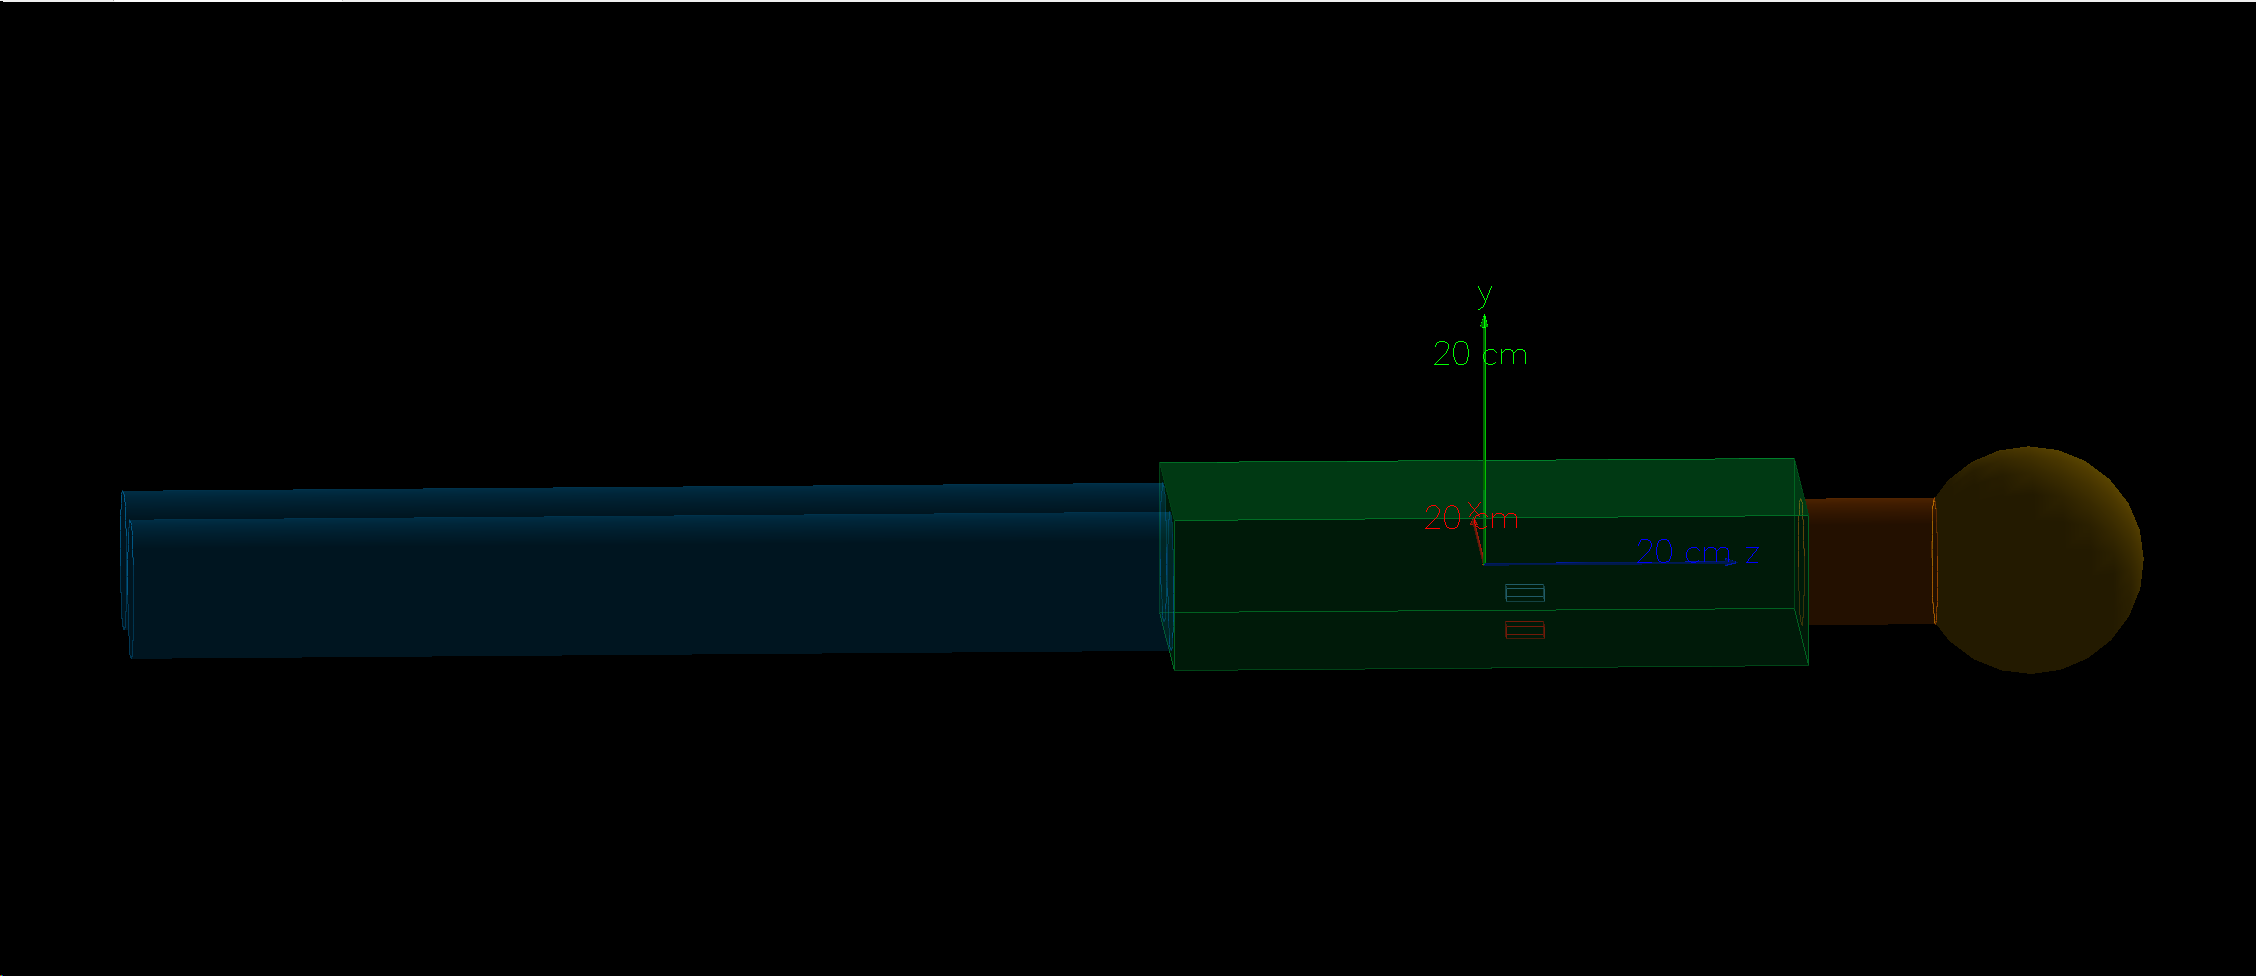
\includegraphics[width=0.78\textwidth]{body.png}
    \caption{Geant4 人体结构可视化}
    \label{fig:body}
\end{figure}

头颈连接处，颈部上端面与头部球面相切，头部采用球体扣除下方球冠的方式避免几何重叠。束流源位于 \verb|(-45, -600, 30) mm|，方向为 \verb|+y|，沿肿瘤中心轴线入射。

\subsection{材料定义}

\begin{table}[H]
    \centering
    \caption{材料定义}
    \label{tab:materials}
    \small
    \begin{tabularx}{\textwidth}{>{\raggedright\arraybackslash}p{2.4cm}>{\raggedright\arraybackslash}p{4.0cm}>{\raggedright\arraybackslash}X}
        \toprule
        材料 & Geant4 定义 & 用途 \\
        \midrule
        空气 & \verb|G4_AIR|（NIST） & World \\
        水 & \verb|G4_WATER|（NIST，\verb|1 g/cm3|） & 人体软组织、无硼区域 \\
        $^{10}\mathrm{B}$ 硼化水 & 自定义 \verb|B10_Borated_Water| & 含硼肿瘤细胞或硼壳层 \\
        \bottomrule
    \end{tabularx}
\end{table}

$^{10}\mathrm{B}$ 同位素参数为 \verb|Z = 5|、\verb|A = 10|、摩尔质量 \verb|10.012937 g/mol|。硼含量用按质量计的 ppm 表示，其中 $1\,\mathrm{ppm}=10^{-6}$ 的质量分数：

\begin{equation}
    \omega_{\mathrm{B}} = C_{\mathrm{B}}(\mathrm{ppm}) \times 10^{-6}.
\end{equation}

Q2 中使用的 $C_{\mathrm{B}}=5.0\times 10^{5}\,\mathrm{ppm}$ 远高于临床 BNCT 中通常讨论的硼浓度范围，对应 $\omega_{\mathrm{B}}=0.5$，即 50\% 质量分数，主要用于在有限事件数下增强反应统计量。

\subsection{辐射剂量说明}

吸收剂量定义为：

\begin{equation}
    D = \frac{E_{\mathrm{dep}}}{m}.
    \label{eq:dose}
\end{equation}

其中，$D$ 为吸收剂量，表示单位质量物质吸收的电离辐射能量；$E_{\mathrm{dep}}$ 为沉积能量，即射线或粒子在特定几何区域内由于相互作用而损失并留在该区域内的总能量；$m$ 为接收该段能量的目标区域质量。

需要注意的是，Q1 和 Q2 的计分尺度不同。Q1 使用宏观区域计分，主要比较 gamma 与 proton 在人体模型中的空间分布形状；Q2 使用整次运行累计的单细胞计分，重点观察含硼细胞与不含硼细胞之间的微观剂量差异。因此，两部分结果可以分别用于讨论剂量分布趋势，但不能直接比较绝对剂量大小。

在 Q1 中，深度剂量曲线和二维热图主要用于观察能量沉积在空间上的分布位置。为了突出曲线形状和热点位置，相关图中的剂量数据进行了归一化处理。LET 谱按每个 step 的 \verb|E_dep / stepLength| 统计，并对 step 数归一化，用来辅助观察不同粒子在肿瘤区内的平均能量损失特征。由于 Q1 事件数有限，LET 结果更适合作为辅助信息，而不是单独作为剂量学判断依据。

在 Q2 中，整细胞剂量由单个球形细胞内累计沉积能量除以细胞质量得到，细胞核剂量则只统计核体积内的沉积能量。计算平均值时，全部 2048 个同类细胞都计入统计，未发生能量沉积的细胞以零剂量参与平均，因此该指标同时受到反应发生概率和单次沉积强度影响。投影热图通过对每个横向坐标 $(x,z)$ 处沿束流方向 $y$ 的细胞剂量进行求和得到，因此反映的是微区在 $x$-$z$ 平面上的累计剂量分布，而不是单一 y 截面的剂量。运行中记录的 $\alpha$ 与 $^{7}\mathrm{Li}$ 二次粒子数之和则作为 BNCT 反应活性的相对指标。

\section{Q1：gamma 与 proton 照射对比}

\subsection{研究目标}

Q1 比较 gamma 与 proton 在宏观人体模型中的剂量沉积差异，重点关注：Bragg peak 是否能落在肿瘤深度附近、入射能量变化对剂量空间分布的影响，以及两种粒子的 LET 谱差异。

相关参数设置如下：

\begin{table}[H]
    \centering
    \caption{Q1 基本照射参数}
    \label{tab:q1-basic}
    \begin{tabular}{lccc}
        \toprule
        粒子 & 能量 & 束斑半径 & 事件数 \\
        \midrule
        gamma & \verb|1 MeV| & \verb|8 mm| & \verb|1000| \\
        proton & \verb|45 MeV| & \verb|8 mm| & \verb|1000| \\
        \bottomrule
    \end{tabular}
\end{table}

能量扫描设置如下：

\begin{table}[H]
    \centering
    \caption{Q1 能量扫描设置}
    \label{tab:q1-scan}
    \small
    \begin{tabularx}{\textwidth}{>{\raggedright\arraybackslash}p{3.0cm}>{\raggedright\arraybackslash}X>{\raggedleft\arraybackslash}p{2.4cm}}
        \toprule
        扫描类型 & 能量点 & 每点事件数 \\
        \midrule
        gamma scan & \verb|0.2, 0.5, 1, 2, 4, 6, 8, 10, 15 MeV| & \verb|1000| \\
        proton scan & \verb|30, 35, 40, 45, 50, 55, 60, 70, 80 MeV| & \verb|500| \\
        \bottomrule
    \end{tabularx}
\end{table}

后续 Q1 的图按照由简单到复杂的顺序展开：先用深度剂量曲线判断剂量峰值是否落在肿瘤所在的 y 范围，再用二维热图检查这种一维观察在躯干投影平面中是否仍然成立；随后通过能量扫描解释峰值或沉积区域为什么会移动，最后用 LET 谱作为对能损特征的补充观察。

\subsection{深度剂量分布}

图\ref{fig:q1-depth-dose}为 gamma 和 proton 沿 y 方向的归一化深度剂量曲线。

\begin{figure}[H]
    \centering
    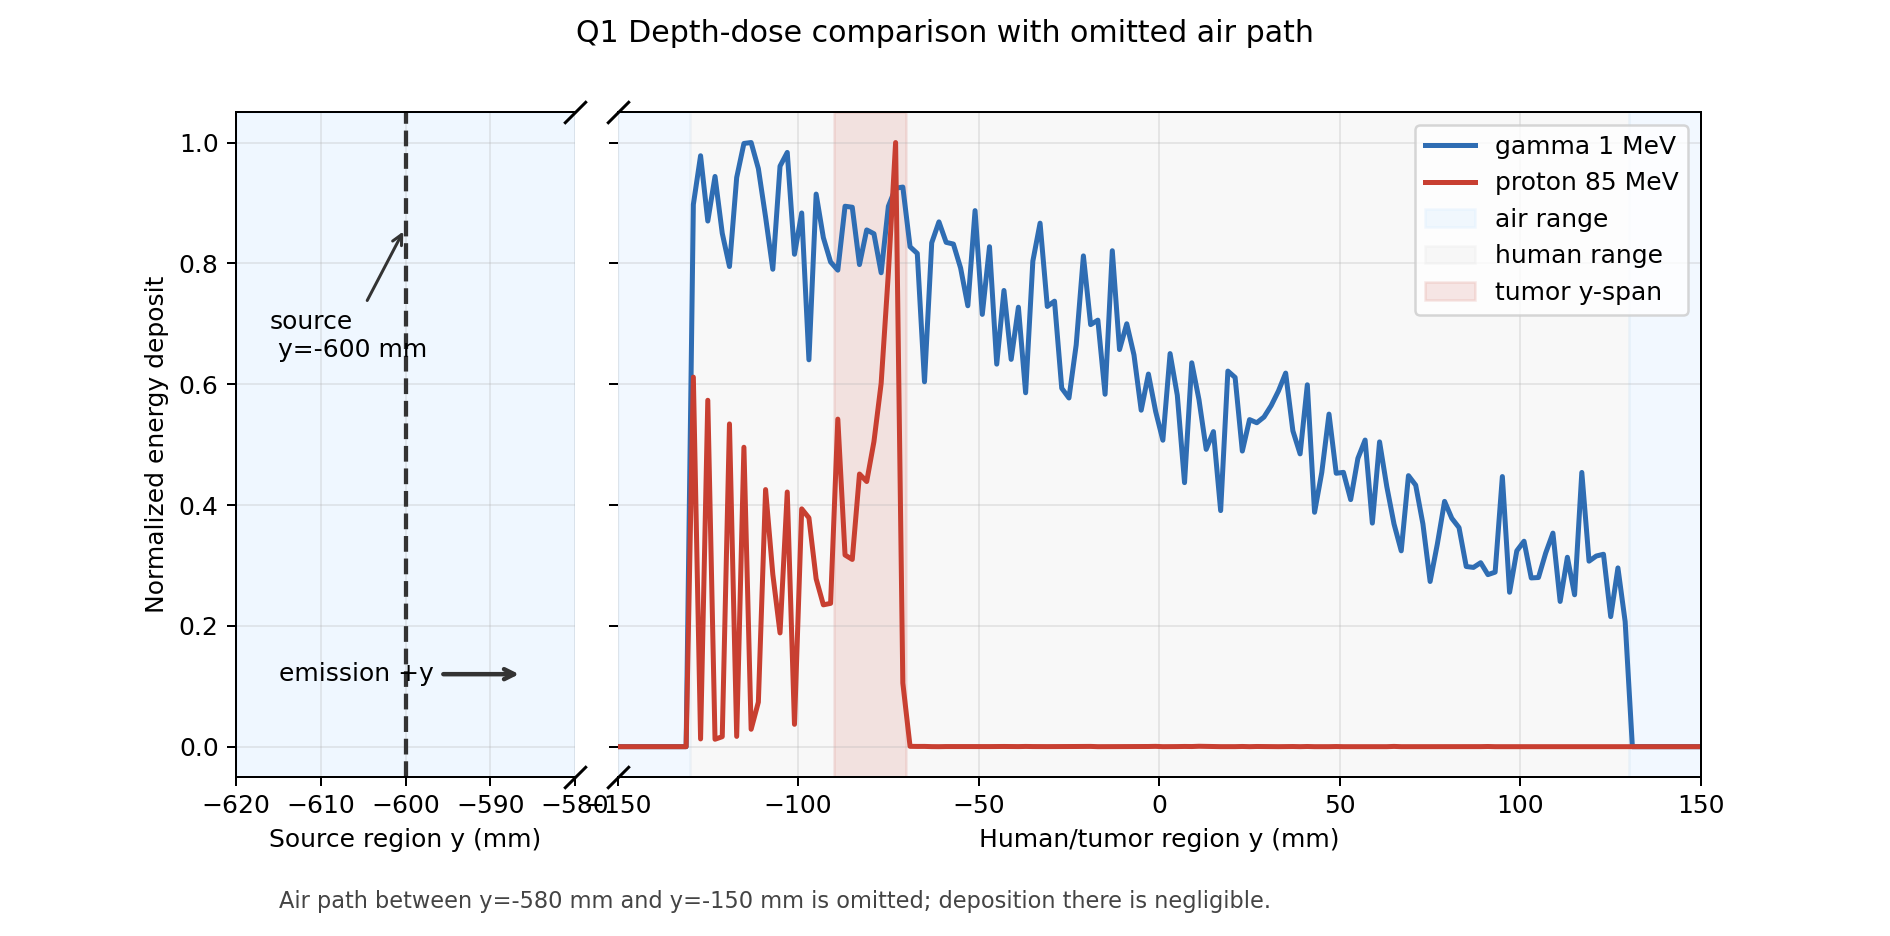
\includegraphics[width=0.85\textwidth]{Q1_depth_dose.png}
    \caption{Q1 gamma 与 proton 深度剂量曲线}
    \label{fig:q1-depth-dose}
\end{figure}

图中 gamma 曲线整体变化较平缓，能量沉积沿入射方向连续分布，没有形成集中的末端峰值。相比之下，45 MeV proton 的归一化剂量在 $y\approx -50\,\mathrm{mm}$ 至 $-40\,\mathrm{mm}$ 附近升高，这一位置接近当前几何中肿瘤区的 y 范围。这个差异说明，在当前简化人体模型中，proton 的剂量分布主要受射程末端 Bragg peak 控制，而 gamma 更接近沿路径连续沉积。

这里的曲线经过归一化处理，主要用于比较两种粒子的空间分布形状，不能直接解释为绝对治疗剂量差异。因此，后文选择 45 MeV proton 作为展示能量，只表示它在本组扫描点中与当前肿瘤深度较匹配。

\subsection{二维剂量热图与肿瘤区设置}

深度剂量曲线只保留了束流方向上的一维信息，还不能显示横向位置和肿瘤边界之间的关系。因此，在确认 proton 峰值接近肿瘤 y 范围后，进一步查看两种粒子在躯干投影平面上的二维能量沉积分布。图\ref{fig:q1-dose-heatmap}中，白色和蓝色边框分别标记躯干与肿瘤区边界。

\begin{figure}[H]
    \centering
    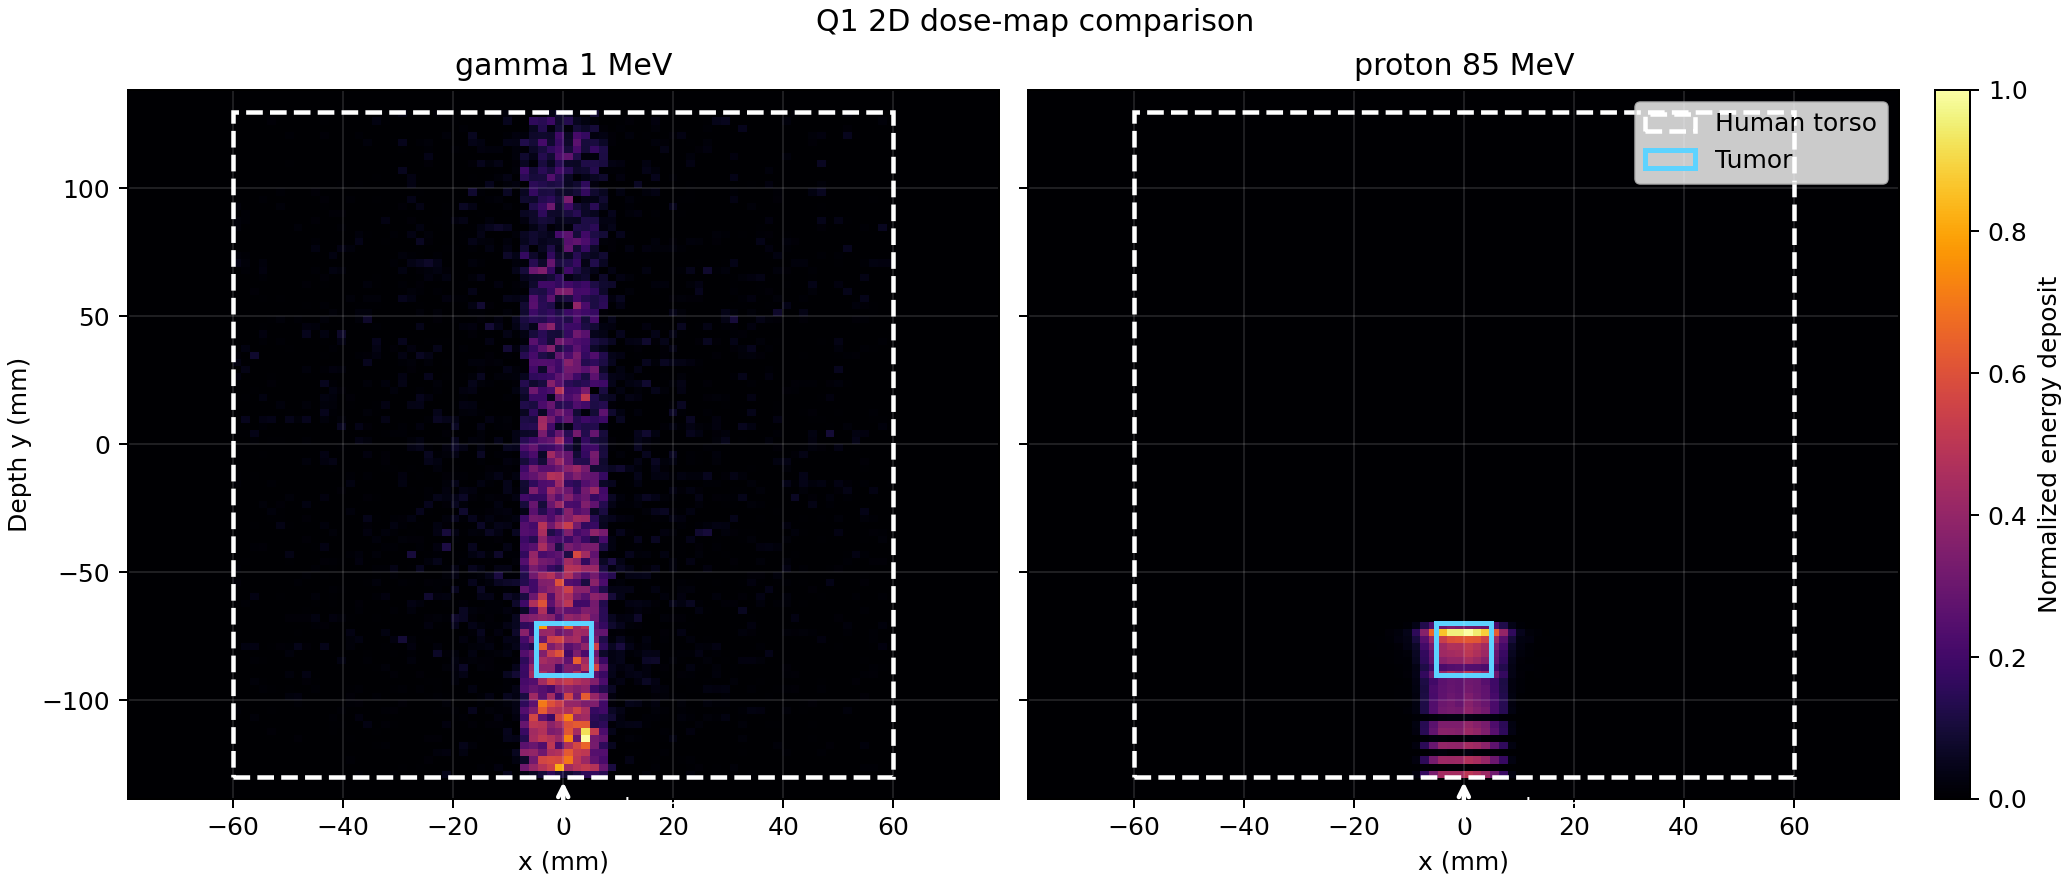
\includegraphics[width=0.88\textwidth]{Q1_dose_heatmap.png}
    \caption{Q1 gamma 与 proton 二维剂量热图}
    \label{fig:q1-dose-heatmap}
\end{figure}

二维热图给出了与深度剂量曲线一致的空间图像。gamma 的沉积分布沿束流路径展开，肿瘤框附近没有形成独立的局部热点；proton 的高剂量区域则更集中在肿瘤位置附近，与图\ref{fig:q1-depth-dose}中 Bragg peak 接近肿瘤深度的结果相对应。

这张图的作用主要是把一维深度曲线转化为更直观的二维空间分布：白色边框显示躯干范围，蓝色边框显示肿瘤区位置。由此可以看到，proton 相对 gamma 的区别并不是简单的“能量更高”，而是在当前能量下末端能量沉积区更容易与肿瘤位置重合。

\subsection{gamma 能量扫描}

前两张图比较的是固定能量下 gamma 与 proton 的差异。为了判断这种差异是否主要来自入射能量选择，后续分别对 gamma 和 proton 做能量扫描。这里先看 gamma，是因为它没有 Bragg peak，可以作为“改变穿透深度但不形成末端峰值”的对照。图\ref{fig:q1-gamma-grid}为不同 gamma 能量下的二维剂量热图网格。

\begin{figure}[htbp]
    \centering
    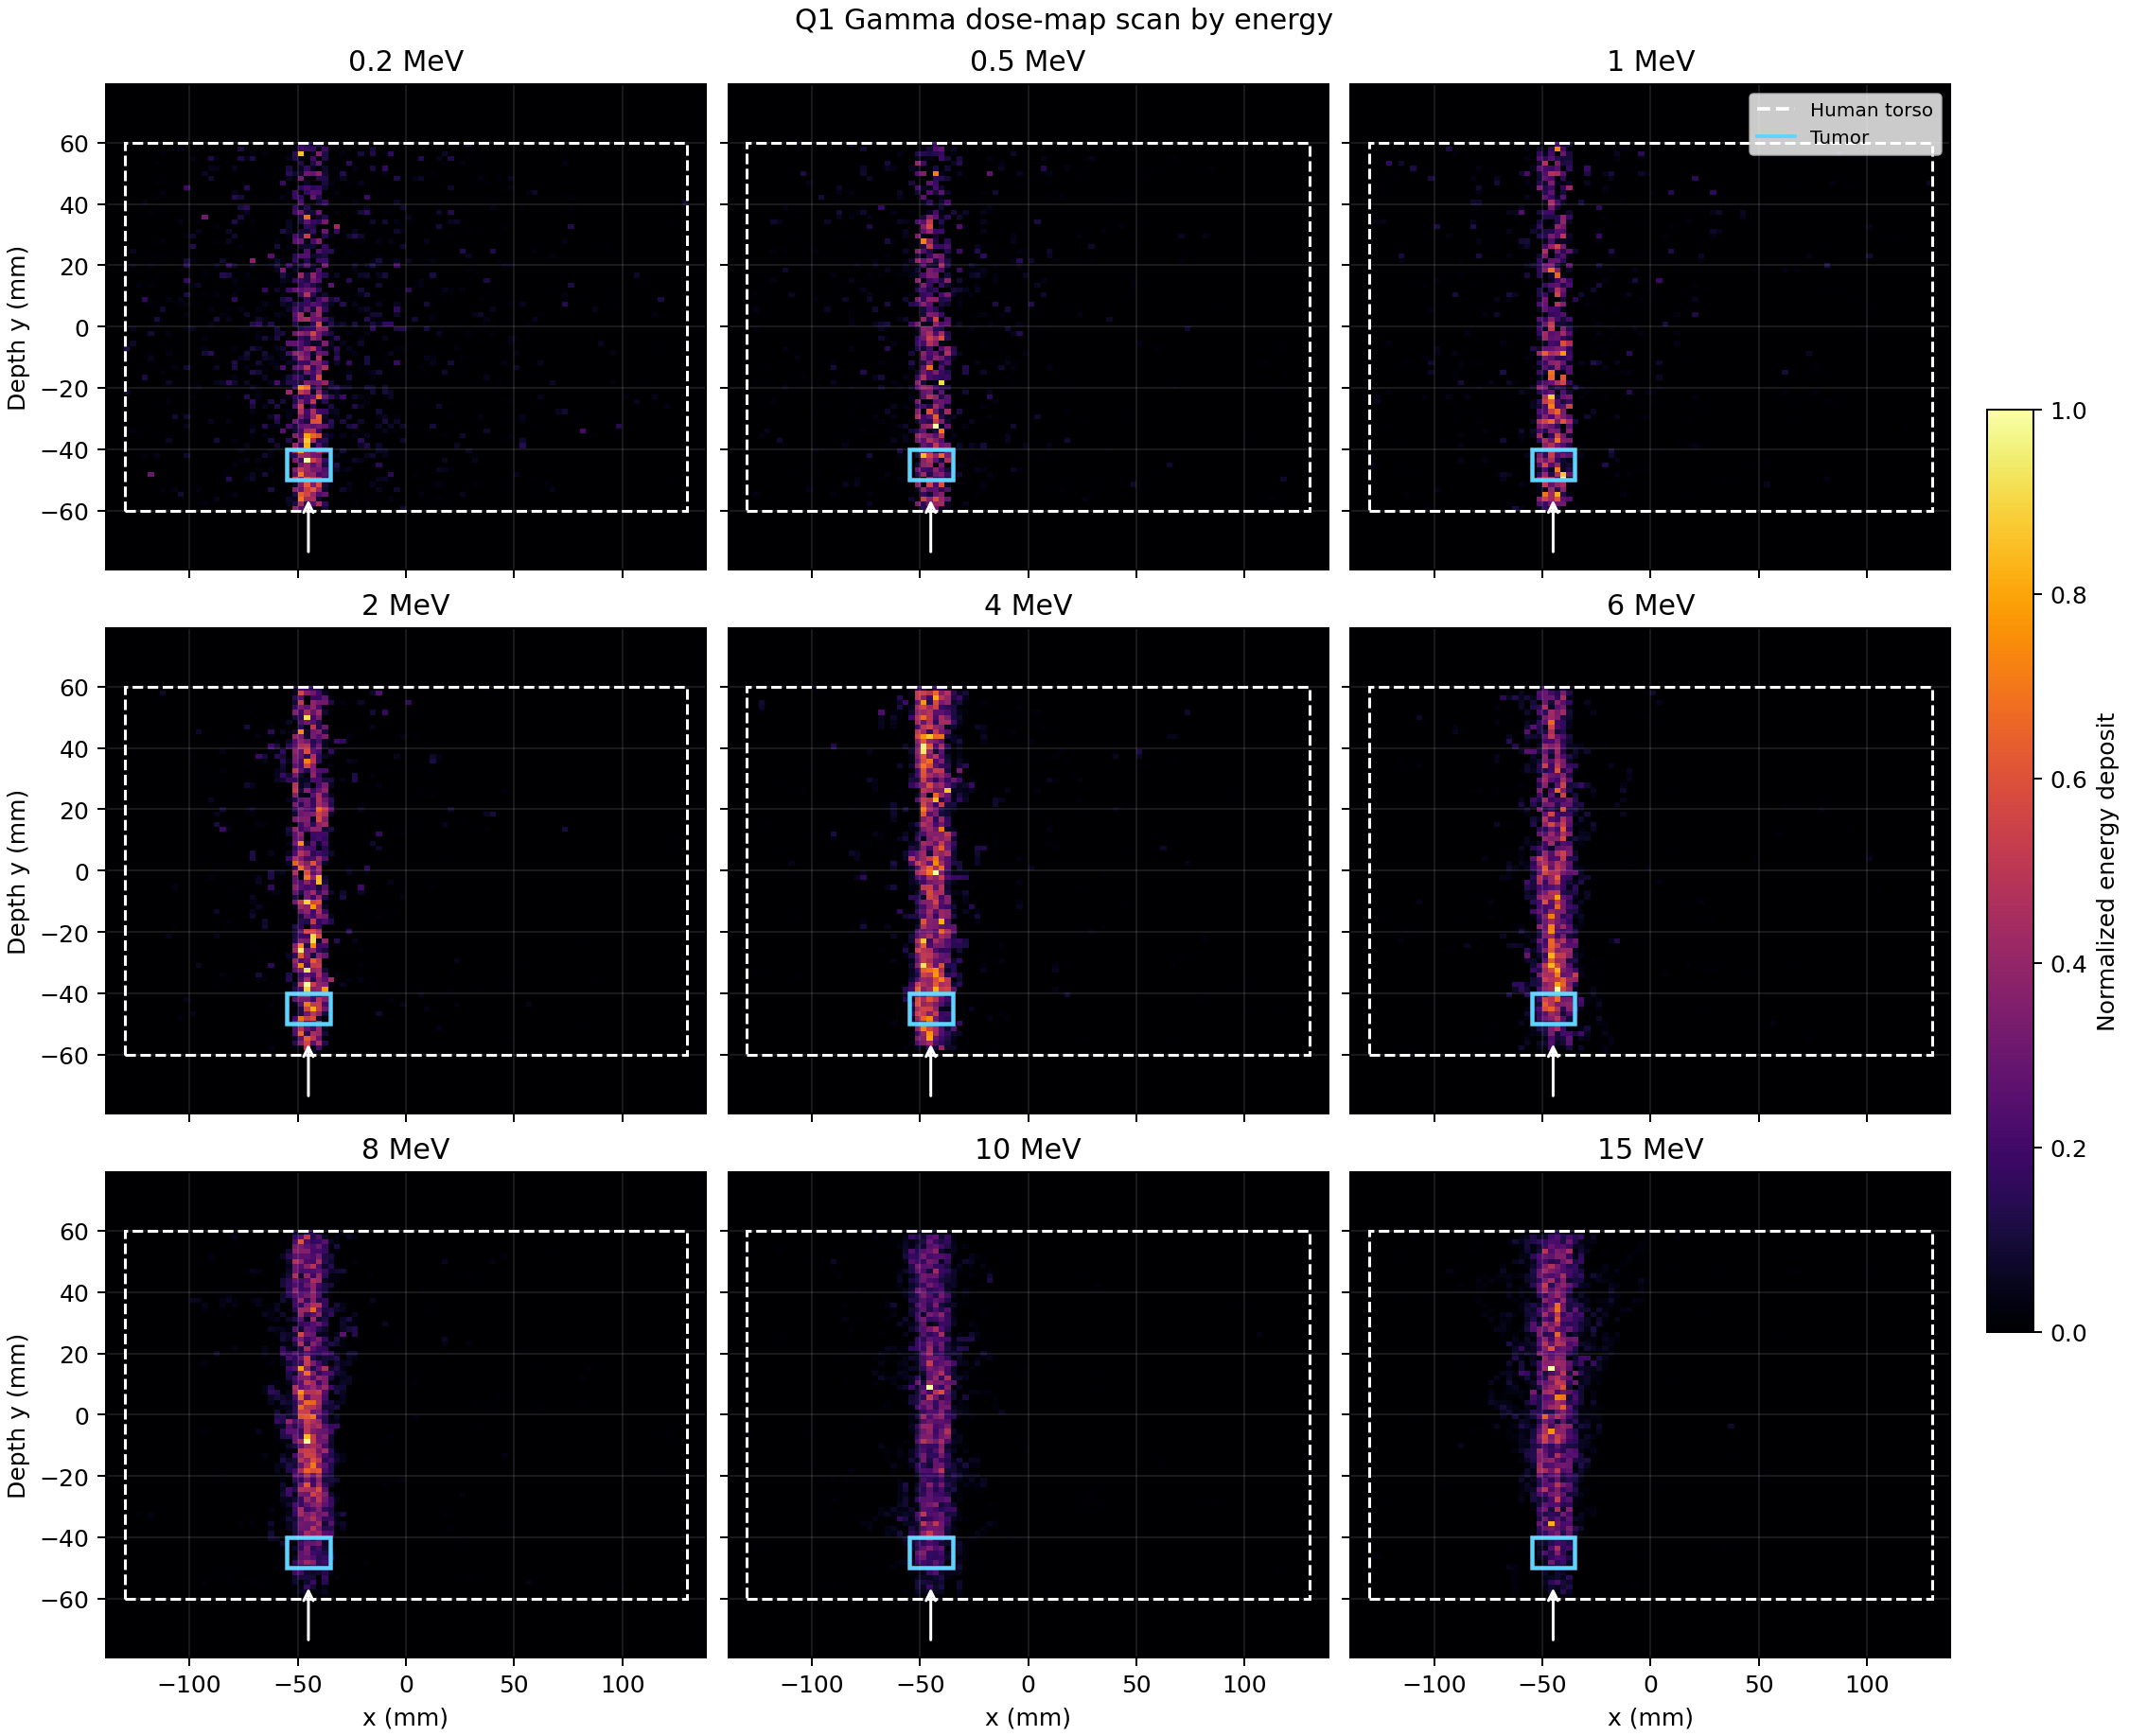
\includegraphics[width=0.65\textwidth]{Q1_gamma_energy_heatmap_grid.png}
    \caption{Q1 gamma 能量二维热图扫描}
    \label{fig:q1-gamma-grid}
\end{figure}

不同 gamma 能量的热图显示，随着入射能量升高，能量沉积区域整体向更深位置延伸，低能 gamma 更容易在较浅区域沉积，高能 gamma 的穿透能力更强。由于 gamma 没有类似质子的 Bragg peak，剂量分布不会在某一深度突然集中，因此热图中主要看到的是穿透深度变化，而不是明确的局部聚焦。

图\ref{fig:q1-gamma-scan}为定量扫描结果，以剂量加权平均深度 \verb|y_mean| 表征整体移动趋势。

\begin{figure}[H]
    \centering
    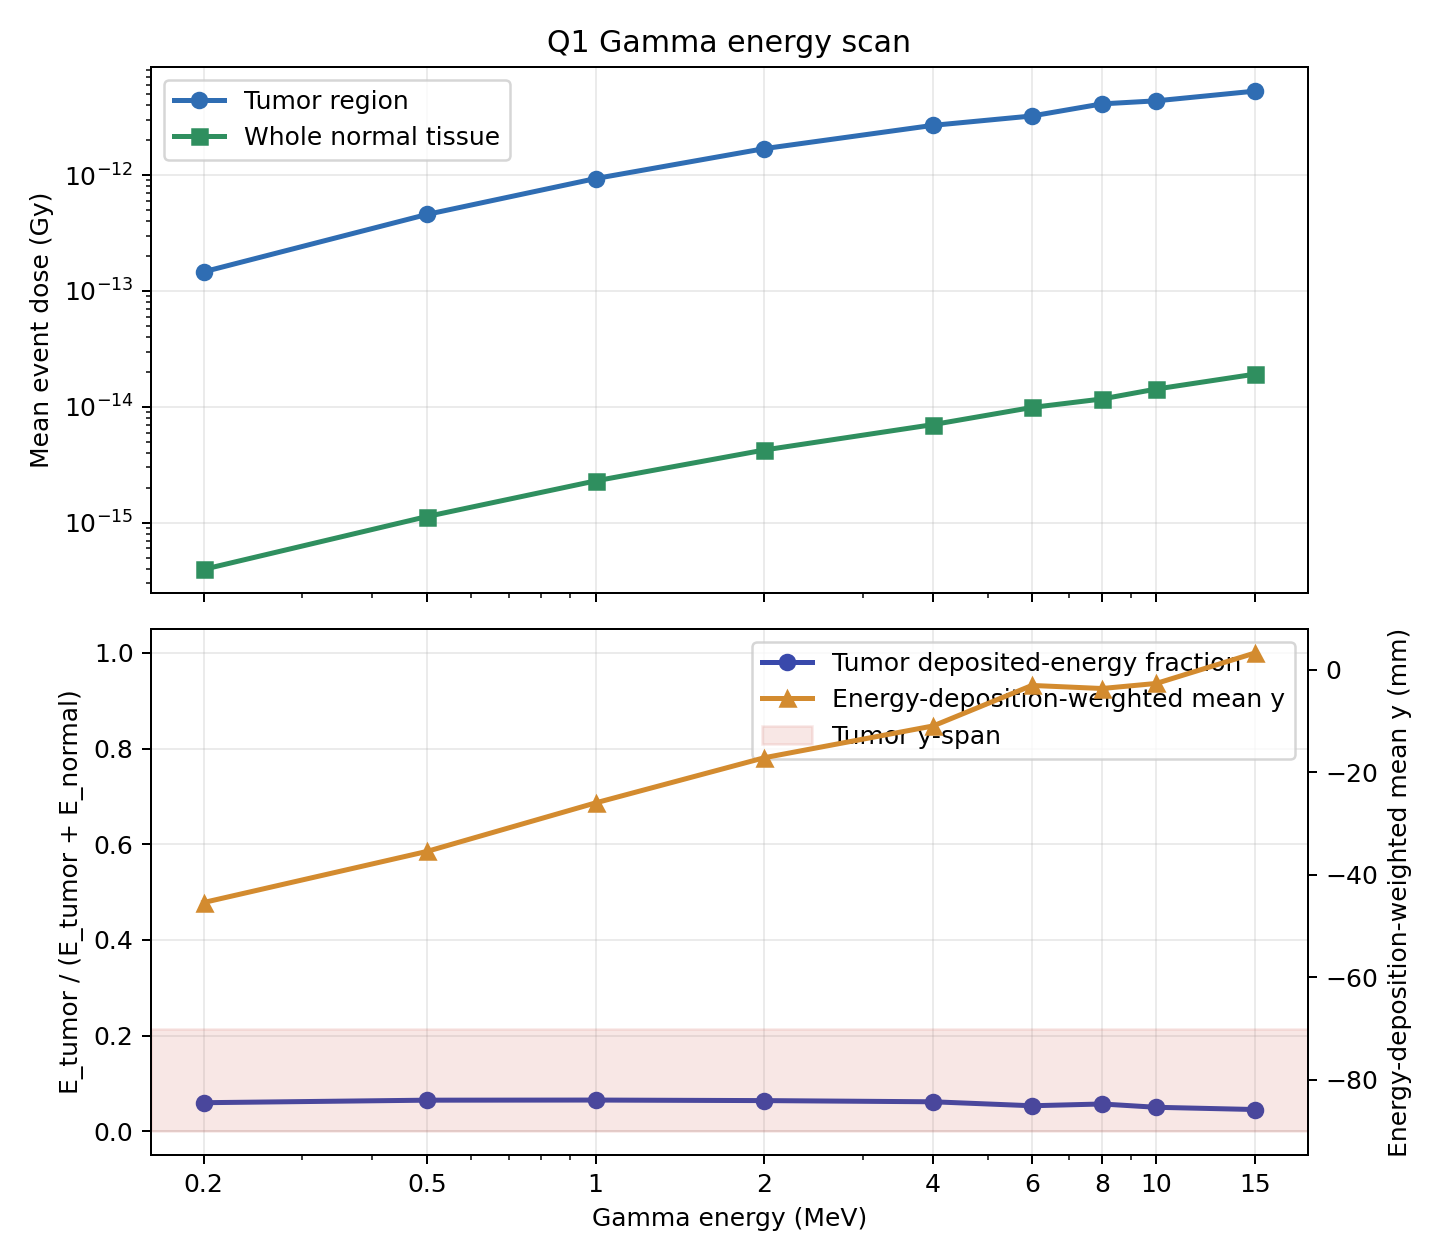
\includegraphics[width=0.88\textwidth]{Q1_gamma_energy_scan.png}
    \caption{Q1 gamma 能量扫描指标}
    \label{fig:q1-gamma-scan}
\end{figure}

定量扫描中的 \verb|y_mean| 也反映了同样的趋势：随 gamma 能量升高，剂量加权平均深度向更深区域移动。但肿瘤沉积能量分数没有随能量升高出现稳定增强，说明在本模型中单纯提高 gamma 能量主要改变穿透能力，并不自动带来更强的肿瘤区选择性。

\subsection{proton 能量扫描}

gamma 扫描说明，提高能量主要改变整体穿透深度；接下来 proton 扫描则用于检查 Bragg peak 是否能通过能量调节与肿瘤深度对齐。因此，这一组图不是单纯重复 gamma 扫描，而是用来寻找当前几何下较匹配的质子能量。图\ref{fig:q1-proton-grid}为不同 proton 能量下的二维剂量热图网格。

\begin{figure}[H]
    \centering
    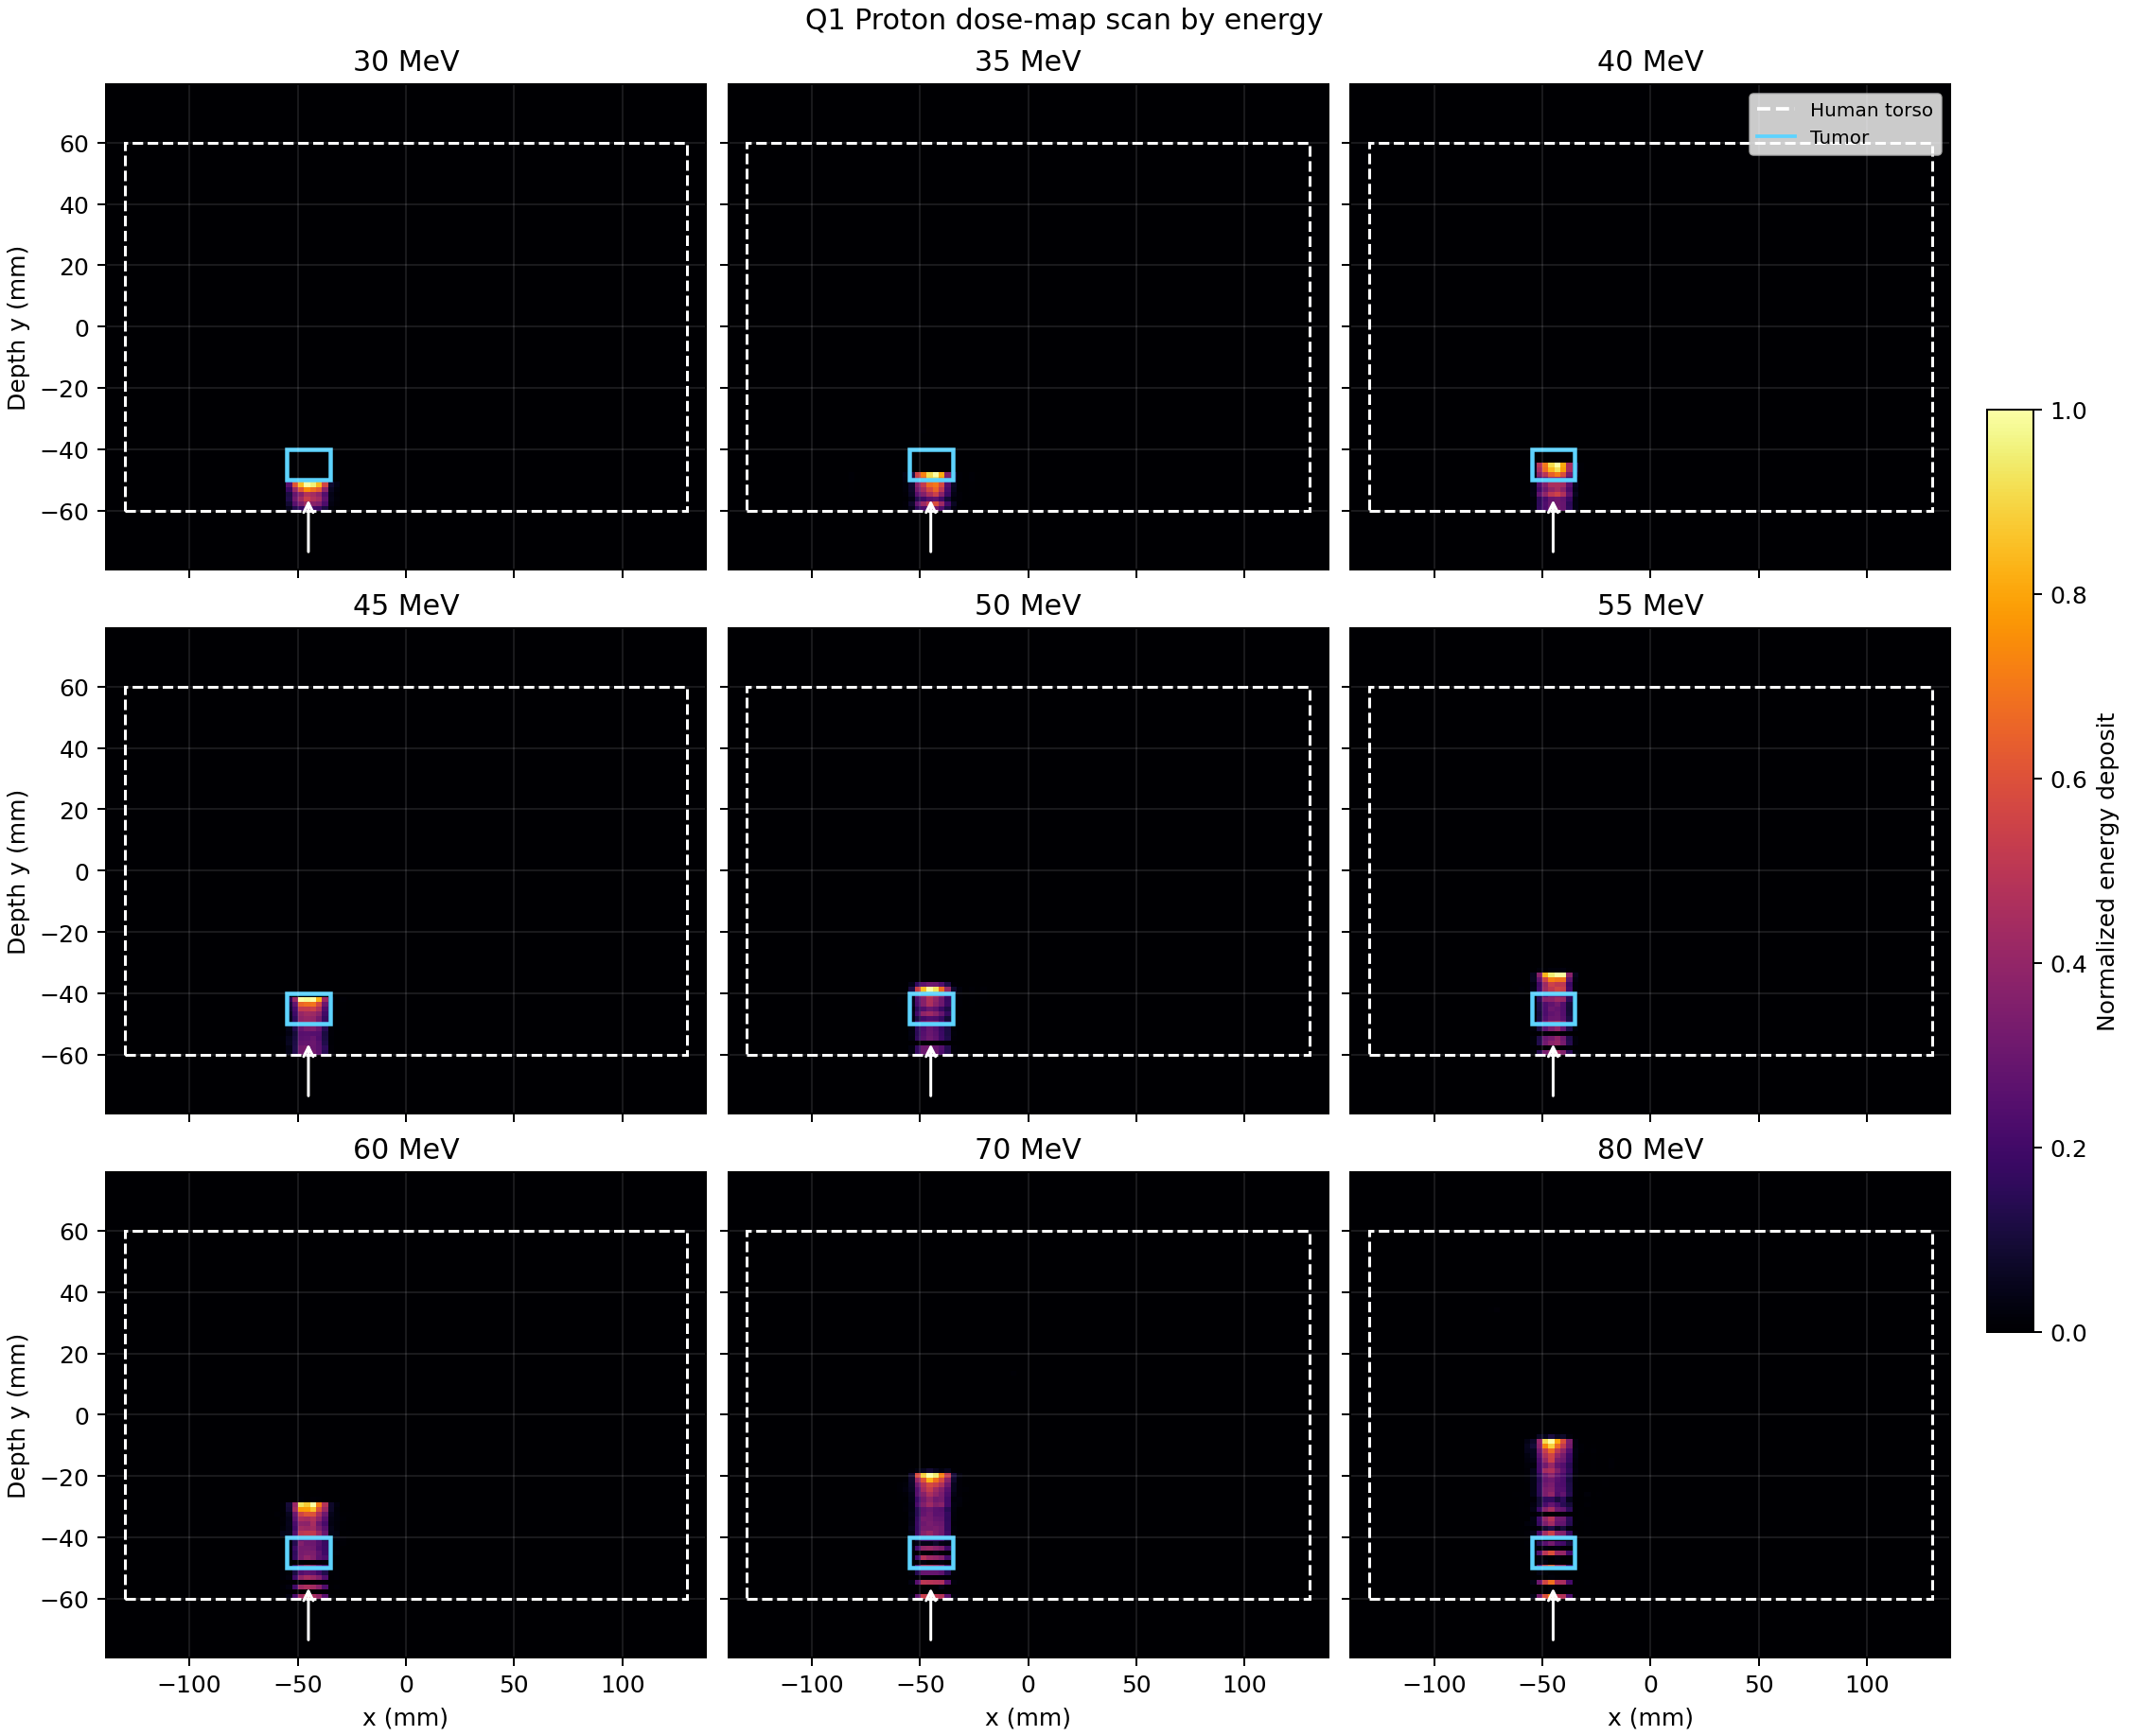
\includegraphics[width=0.95\textwidth]{Q1_proton_energy_heatmap_grid.png}
    \caption{Q1 proton 能量二维热图扫描}
    \label{fig:q1-proton-grid}
\end{figure}

质子能量扫描的变化更接近“峰位移动”的问题。随质子能量升高，Bragg peak 沿束流方向向下游移动：能量过低时，峰值停在肿瘤之前的较浅位置；能量过高时，峰值可能越过肿瘤区。与 gamma 扫描相比，proton 扫描的关键不只是穿透深度增加，而是寻找峰值位置与肿瘤深度的匹配关系。

图\ref{fig:q1-proton-scan}为定量指标，关键指标为肿瘤沉积能量分数：

\begin{equation}
    \omega_E = \frac{E_{\mathrm{tumor}}}{E_{\mathrm{tumor}} + E_{\mathrm{normal}}}.
\end{equation}

\begin{figure}[H]
    \centering
    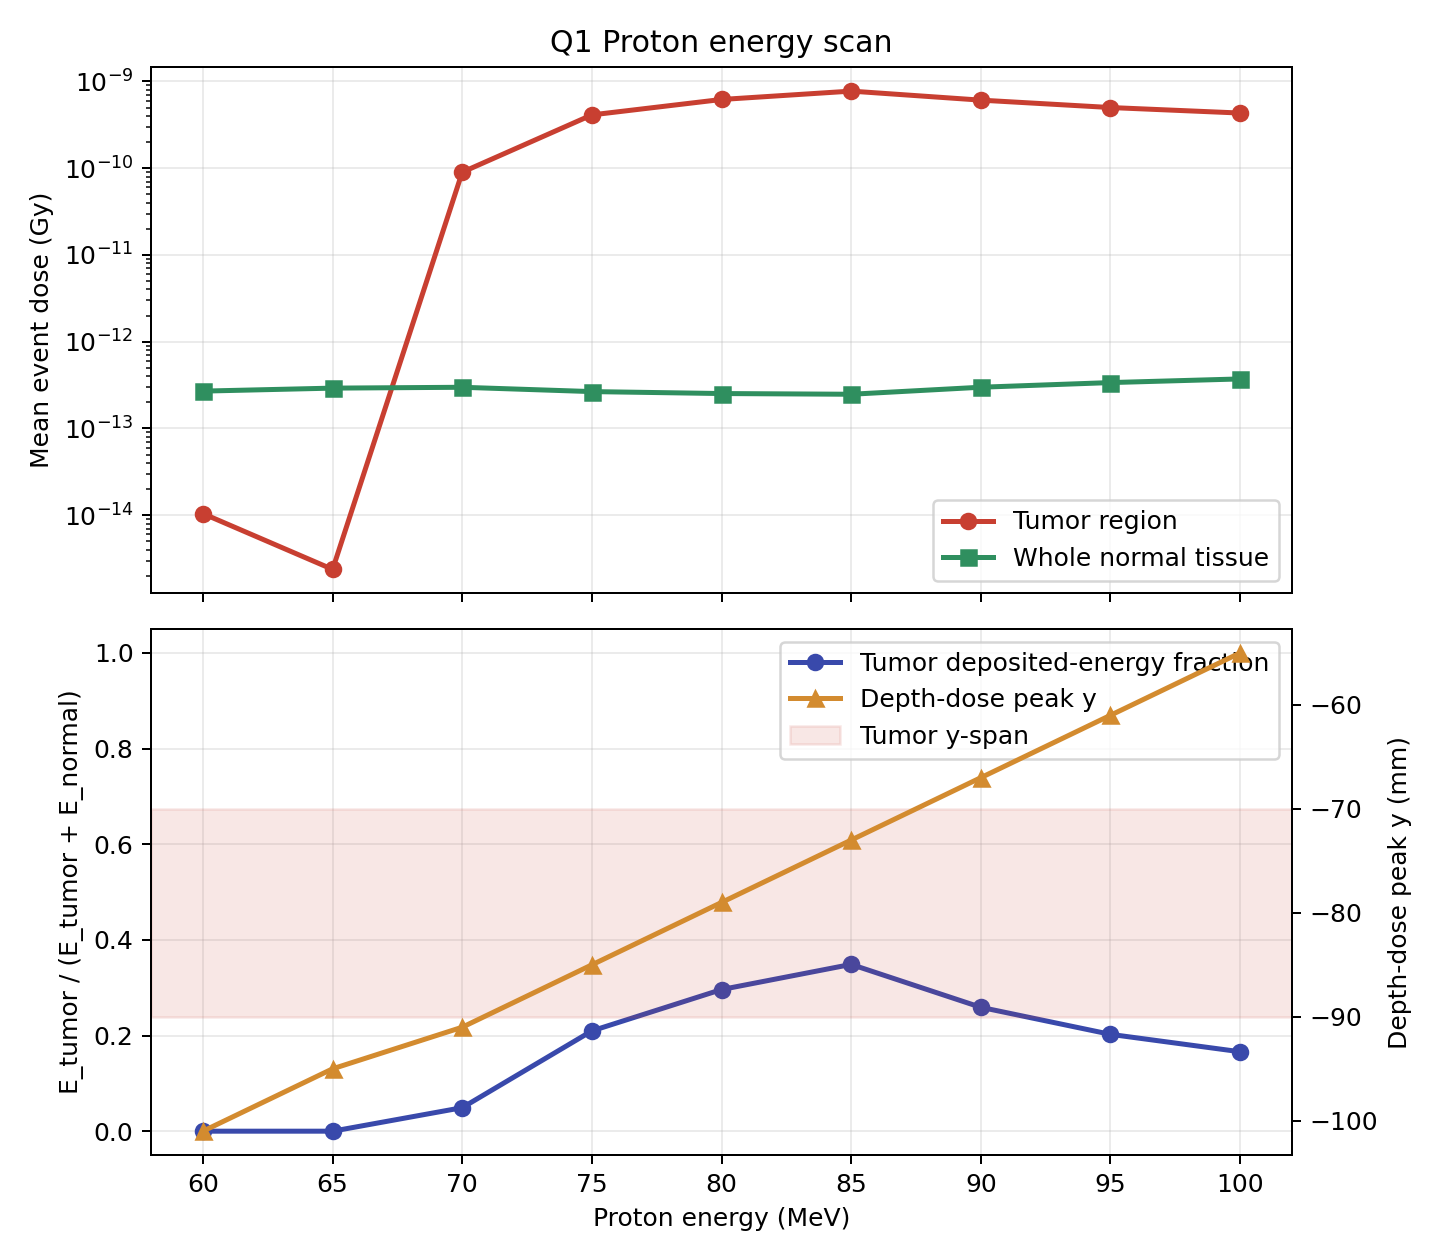
\includegraphics[width=0.88\textwidth]{Q1_proton_energy_scan.png}
    \caption{Q1 proton 能量扫描指标}
    \label{fig:q1-proton-scan}
\end{figure}

扫描结果显示，45 MeV 质子在当前几何中该分数较高，是本组扫描点中较合适的展示能量。这个判断依赖于本报告设置的肿瘤位置、束流方向和扫描能量点；如果肿瘤深度或人体几何改变，匹配能量也需要重新扫描。

\subsection{LET 谱比较}

前面的深度剂量和热图主要回答“能量沉积在哪里”，能量扫描进一步说明“峰值位置如何随入射能量改变”。LET 谱则从另一个角度观察肿瘤区内的能量损失方式，用来辅助判断 proton 在接近射程末端时是否表现出更集中的能损。图\ref{fig:q1-let}为 gamma 与 proton 在肿瘤区内的 LET 谱，横轴限制在 $0$--$2\,\mathrm{MeV}/\mu\mathrm{m}$。

\begin{figure}[H]
    \centering
    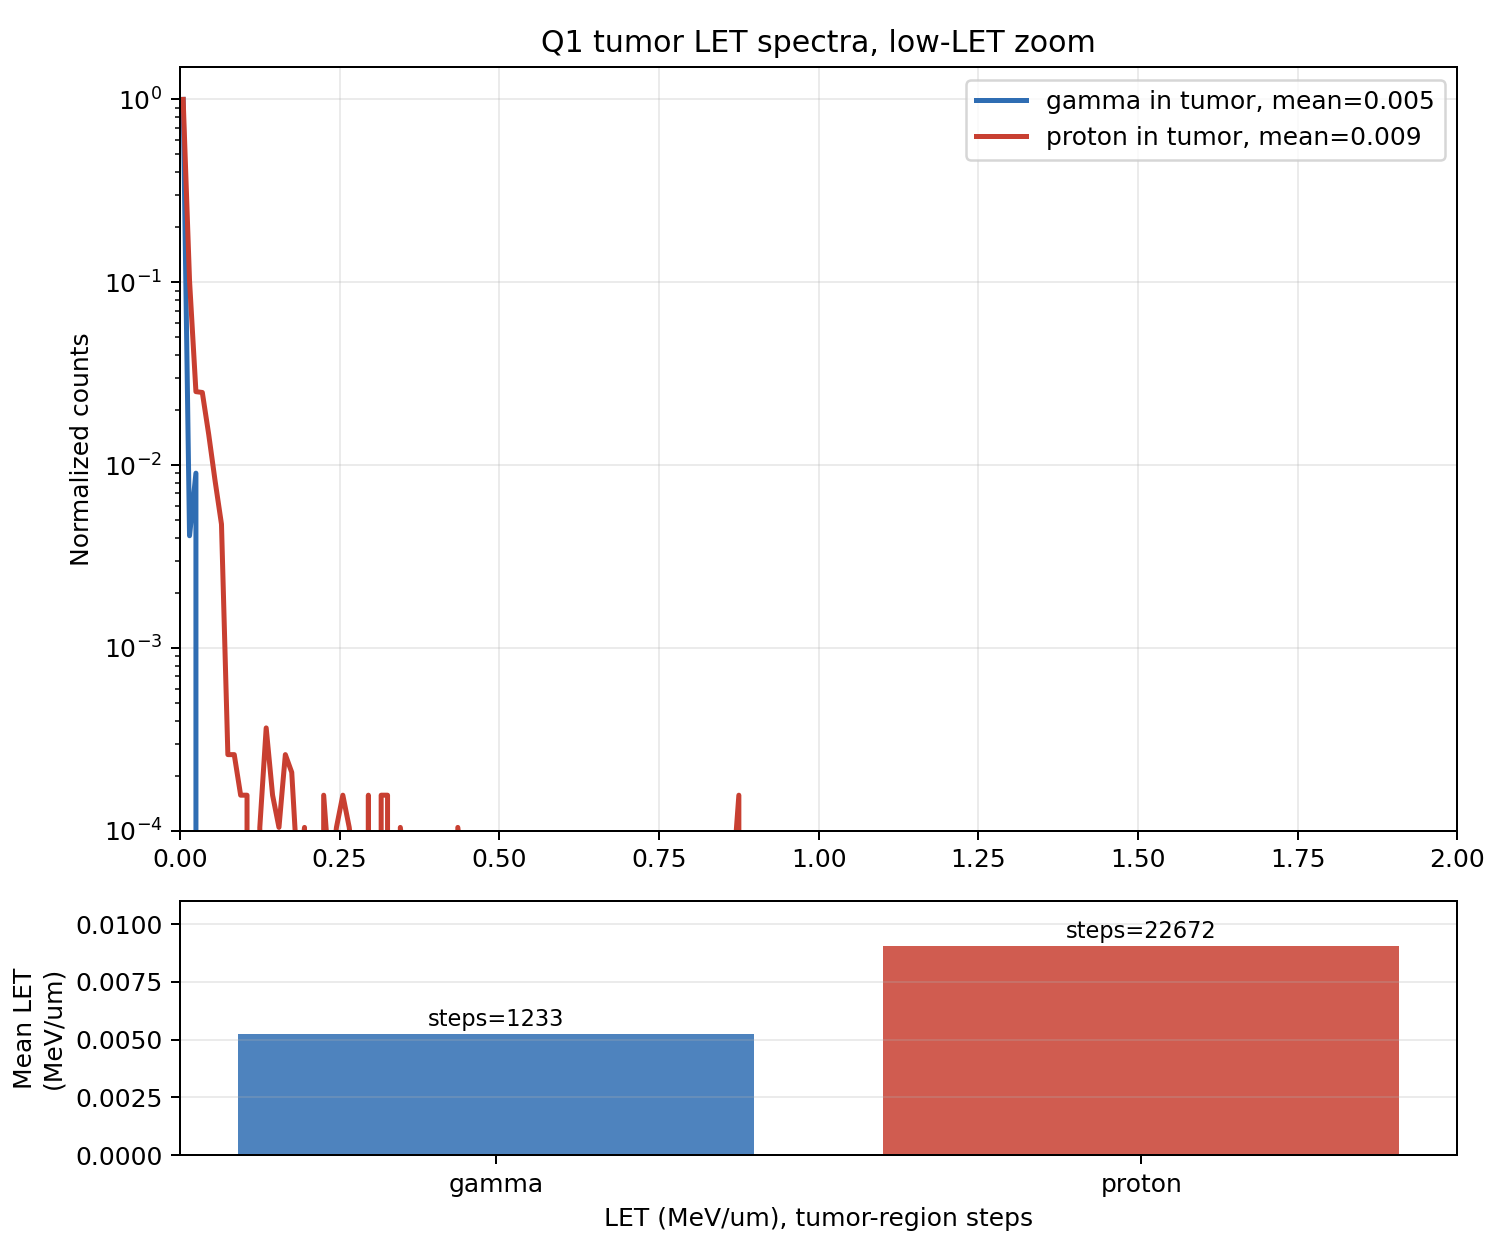
\includegraphics[width=0.86\textwidth]{Q1_let_spectra.png}
    \caption{Q1 肿瘤区 LET 谱}
    \label{fig:q1-let}
\end{figure}

proton 的 step-LET 谱尾部更长，按 step 统计的平均值高于 gamma，反映质子在接近射程末端时单位长度能量损失更集中。这一点与前面深度剂量曲线和热图中观察到的局部沉积相互呼应。不过 LET 谱对 step 统计和事件数较敏感，因此本报告只把它作为辅助判断，Q1 的主要结论仍来自深度剂量曲线、二维热图和能量扫描。

\subsection{Q1 小结}

本次模拟中，gamma 的剂量分布主要表现为沿入射路径的弥散沉积，能量扫描更多改变的是穿透深度；proton 的峰值位置则会随能量变化沿束流方向移动，因此可以通过扫描寻找与肿瘤深度较匹配的能量点。45 MeV 在当前几何中使 Bragg peak 接近肿瘤深度，所以被选作后续展示点。LET 结果与这一观察方向一致，但由于统计量有限，本节的主要判断仍以深度剂量曲线、二维热图和能量扫描为依据。

\section{Q2：BNCT 细胞尺度模拟}

\subsection{研究目标}

BNCT 通过含硼载体药物使肿瘤细胞选择性富集 $^{10}\mathrm{B}$，再用低能中子照射；本模型中将中子能量设为 \verb|0.5 eV|，用于触发以下俘获反应：

\begin{equation}
    ^{10}\mathrm{B} + n \rightarrow \alpha + ^{7}\mathrm{Li}.
\end{equation}

反应产物 $\alpha$ 和 $^{7}\mathrm{Li}$ 射程仅约 $10\,\mu\mathrm{m}$，能量主要沉积在含硼细胞及其近邻区域，因此在模型中预期会出现更局部的能量沉积。

Q2 的目标是：在同一中子场内，比较 $^{10}\mathrm{B}$ 均匀分布与壳层分布两种情形下，含硼肿瘤细胞与不含硼对照细胞的整细胞剂量、细胞核剂量和 $\alpha$+$^{7}\mathrm{Li}$ 产额差异，并通过 $^{10}\mathrm{B}$ 浓度和中子注量扫描分别分析两个参数的作用。

因此，Q2 的图表顺序先从模型本身开始：先说明细胞如何排列，再说明 $^{10}\mathrm{B}$ 放在细胞的什么位置；在几何和材料分布固定后，先比较 uniform 与 shell 的固定浓度结果，再分别改变 $^{10}\mathrm{B}$ 浓度和中子注量，最后把 BNCT 与 gamma/proton 放在同一细胞 patch 下做机制对照。

\subsection{混合细胞模型}

在宏观肿瘤区内设置一个代表性采样，而非将整个厘米量级的肿瘤区全部离散为微米尺度细胞（计算量过大），参数如下：

\begin{table}[H]
    \centering
    \caption{Q2 混合细胞模型参数}
    \label{tab:q2-cell-model}
    \begin{tabular}{lc}
        \toprule
        参数 & 数值 \\
        \midrule
        采样尺寸 & \verb|200 um x 200 um x 200 um| \\
        细胞中心间距 & \verb|12 um| \\
        细胞直径 & \verb|10 um| \\
        细胞核半径 & \verb|2.5 um| \\
        shell 模式硼壳层厚度 & \verb|1 um| \\
        总细胞数 & \verb|4096|（肿瘤细胞 2048，对照细胞 2048） \\
        \bottomrule
    \end{tabular}
\end{table}

混合排列方式如图\ref{fig:q2-layout}所示，红色为含 $^{10}\mathrm{B}$ 肿瘤细胞，绿色为无 $^{10}\mathrm{B}$ 正常细胞。

\begin{figure}[H]
    \centering
    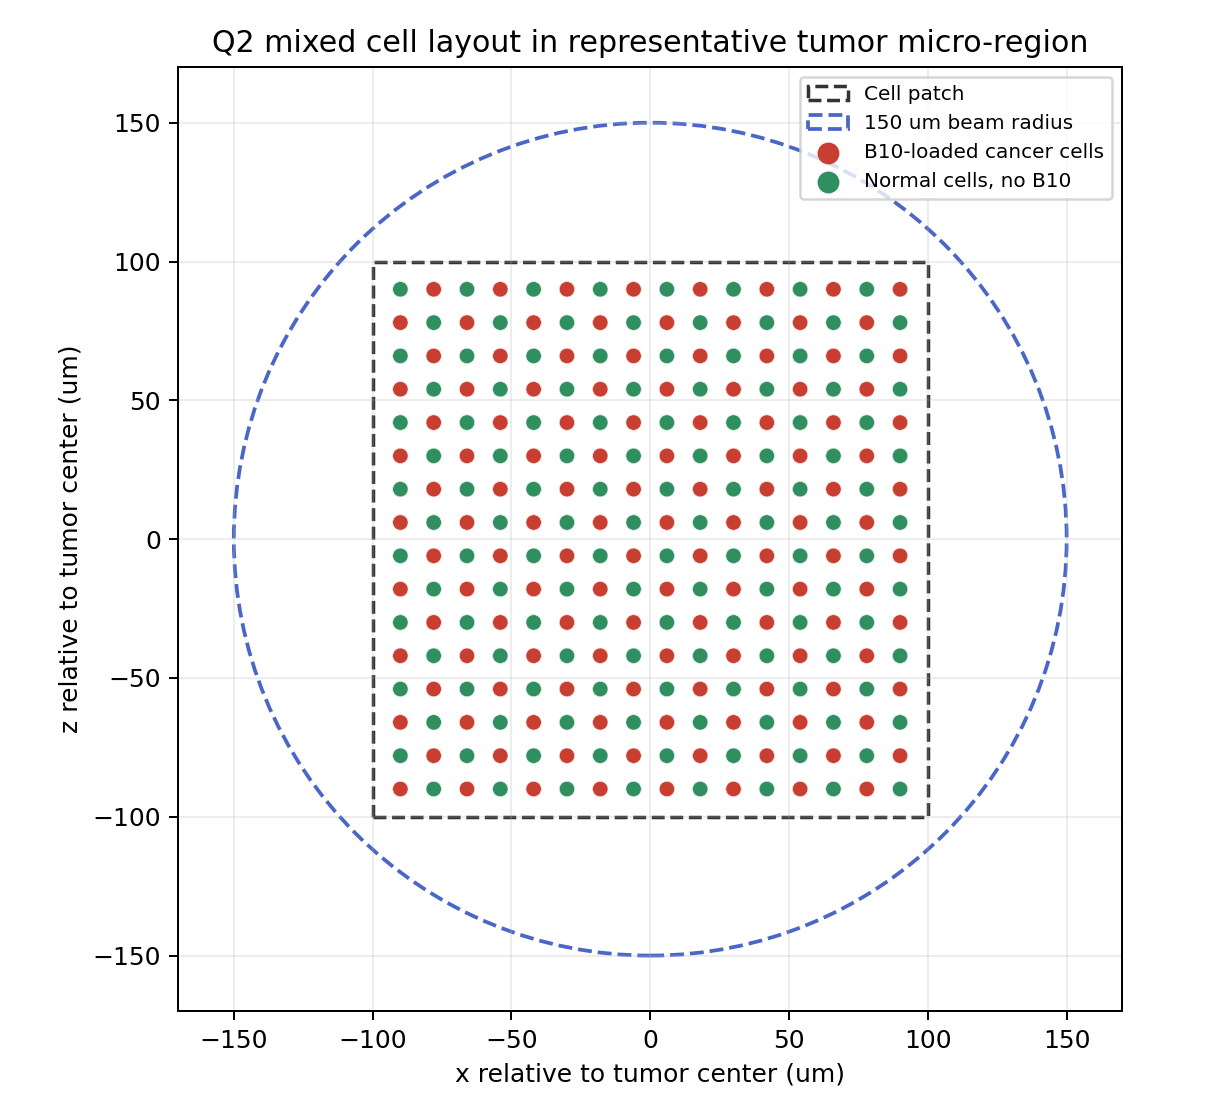
\includegraphics[width=0.82\textwidth]{Q2_geometry_mixed_cell_layout.png}
    \caption{Q2 代表性肿瘤微区混合细胞排列}
    \label{fig:q2-layout}
\end{figure}

两类细胞位于同一微区和同一中子场内，后续剂量差异主要反映 $^{10}\mathrm{B}$ 富集的影响，而非空间位置差异。为了使投影图中的红/绿细胞类型保持清晰，同一横向坐标 $(x,z)$ 上沿束流方向排列的细胞被设置为相同类型，最终在 $x$-$z$ 平面上形成交错分布。

\subsection{\texorpdfstring{$^{10}\mathrm{B}$}{10B} 分布模式}

在确定混合细胞排列后，下一步需要说明含硼肿瘤细胞内部的 $^{10}\mathrm{B}$ 如何放置。这个设置会直接影响短射程二次粒子离细胞核的距离，因此是后续比较整细胞剂量和细胞核剂量的前提。比较两种 $^{10}\mathrm{B}$ 分布模式，示意见图\ref{fig:q2-boron-model}。

\begin{figure}[H]
    \centering
    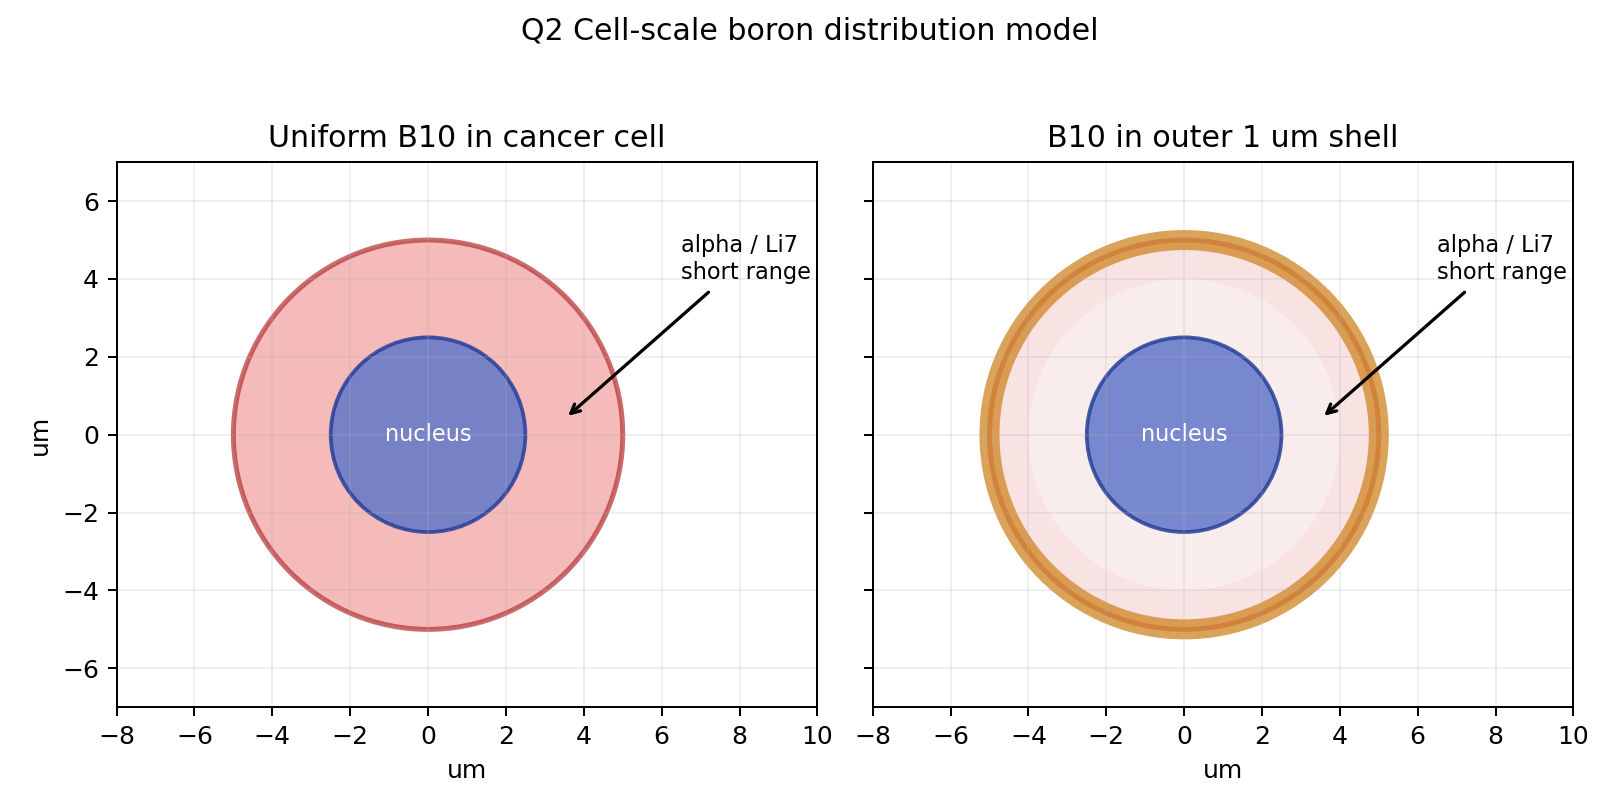
\includegraphics[width=0.82\textwidth]{Q2_boron_distribution_cell_model.png}
    \caption{Q2 $^{10}\mathrm{B}$ 在肿瘤细胞中的分布模式}
    \label{fig:q2-boron-model}
\end{figure}

\begin{table}[H]
    \centering
    \caption{$^{10}\mathrm{B}$ 分布模式}
    \label{tab:q2-boron-mode}
    \small
    \begin{tabularx}{\textwidth}{>{\raggedright\arraybackslash}p{2.2cm}>{\raggedright\arraybackslash}X>{\raggedright\arraybackslash}X}
        \toprule
        模式 & 定义 & 物理含义 \\
        \midrule
        uniform & 整个肿瘤细胞（含细胞核）均匀含 $^{10}\mathrm{B}$ & $^{10}\mathrm{B}$ 进入细胞内部 \\
        shell & $^{10}\mathrm{B}$ 集中在细胞外侧 \verb|1 um| 壳层 & $^{10}\mathrm{B}$ 偏向细胞膜或细胞外周区域 \\
        \bottomrule
    \end{tabularx}
\end{table}

相关参数设置如下：

\begin{table}[H]
    \centering
    \caption{Q2 BNCT 基本参数}
    \label{tab:q2-basic}
    \begin{tabular}{lc}
        \toprule
        参数 & 数值 \\
        \midrule
        中子能量 & \verb|0.5 eV| \\
        束斑半径 & \verb|150 um| \\
        $^{10}\mathrm{B}$ 浓度 & \verb|500000 ppm| \\
        每组事件数 & \verb|20000| \\
        \bottomrule
    \end{tabular}
\end{table}

\subsection{固定浓度下的剂量沉积比较}

前两节已经固定了“细胞怎么排”和“硼怎么放”。在此基础上，先不改变浓度和中子注量，而是在同一组高统计量条件下直接比较 uniform 与 shell，这样可以把观察重点集中在 $^{10}\mathrm{B}$ 空间分布本身。为了深入对比两种不同的硼形态（均匀分布模式 uniform 与细胞膜/外壳分布模式 shell）对微观剂量的影响，本节采用高统计量（20 万个入射粒子）的模拟结果进行分析。

图\ref{fig:q2-micro-dose}展示了两种模式下，细胞在 y 方向投影的剂量热力图。

\begin{figure}[H]
    \centering
    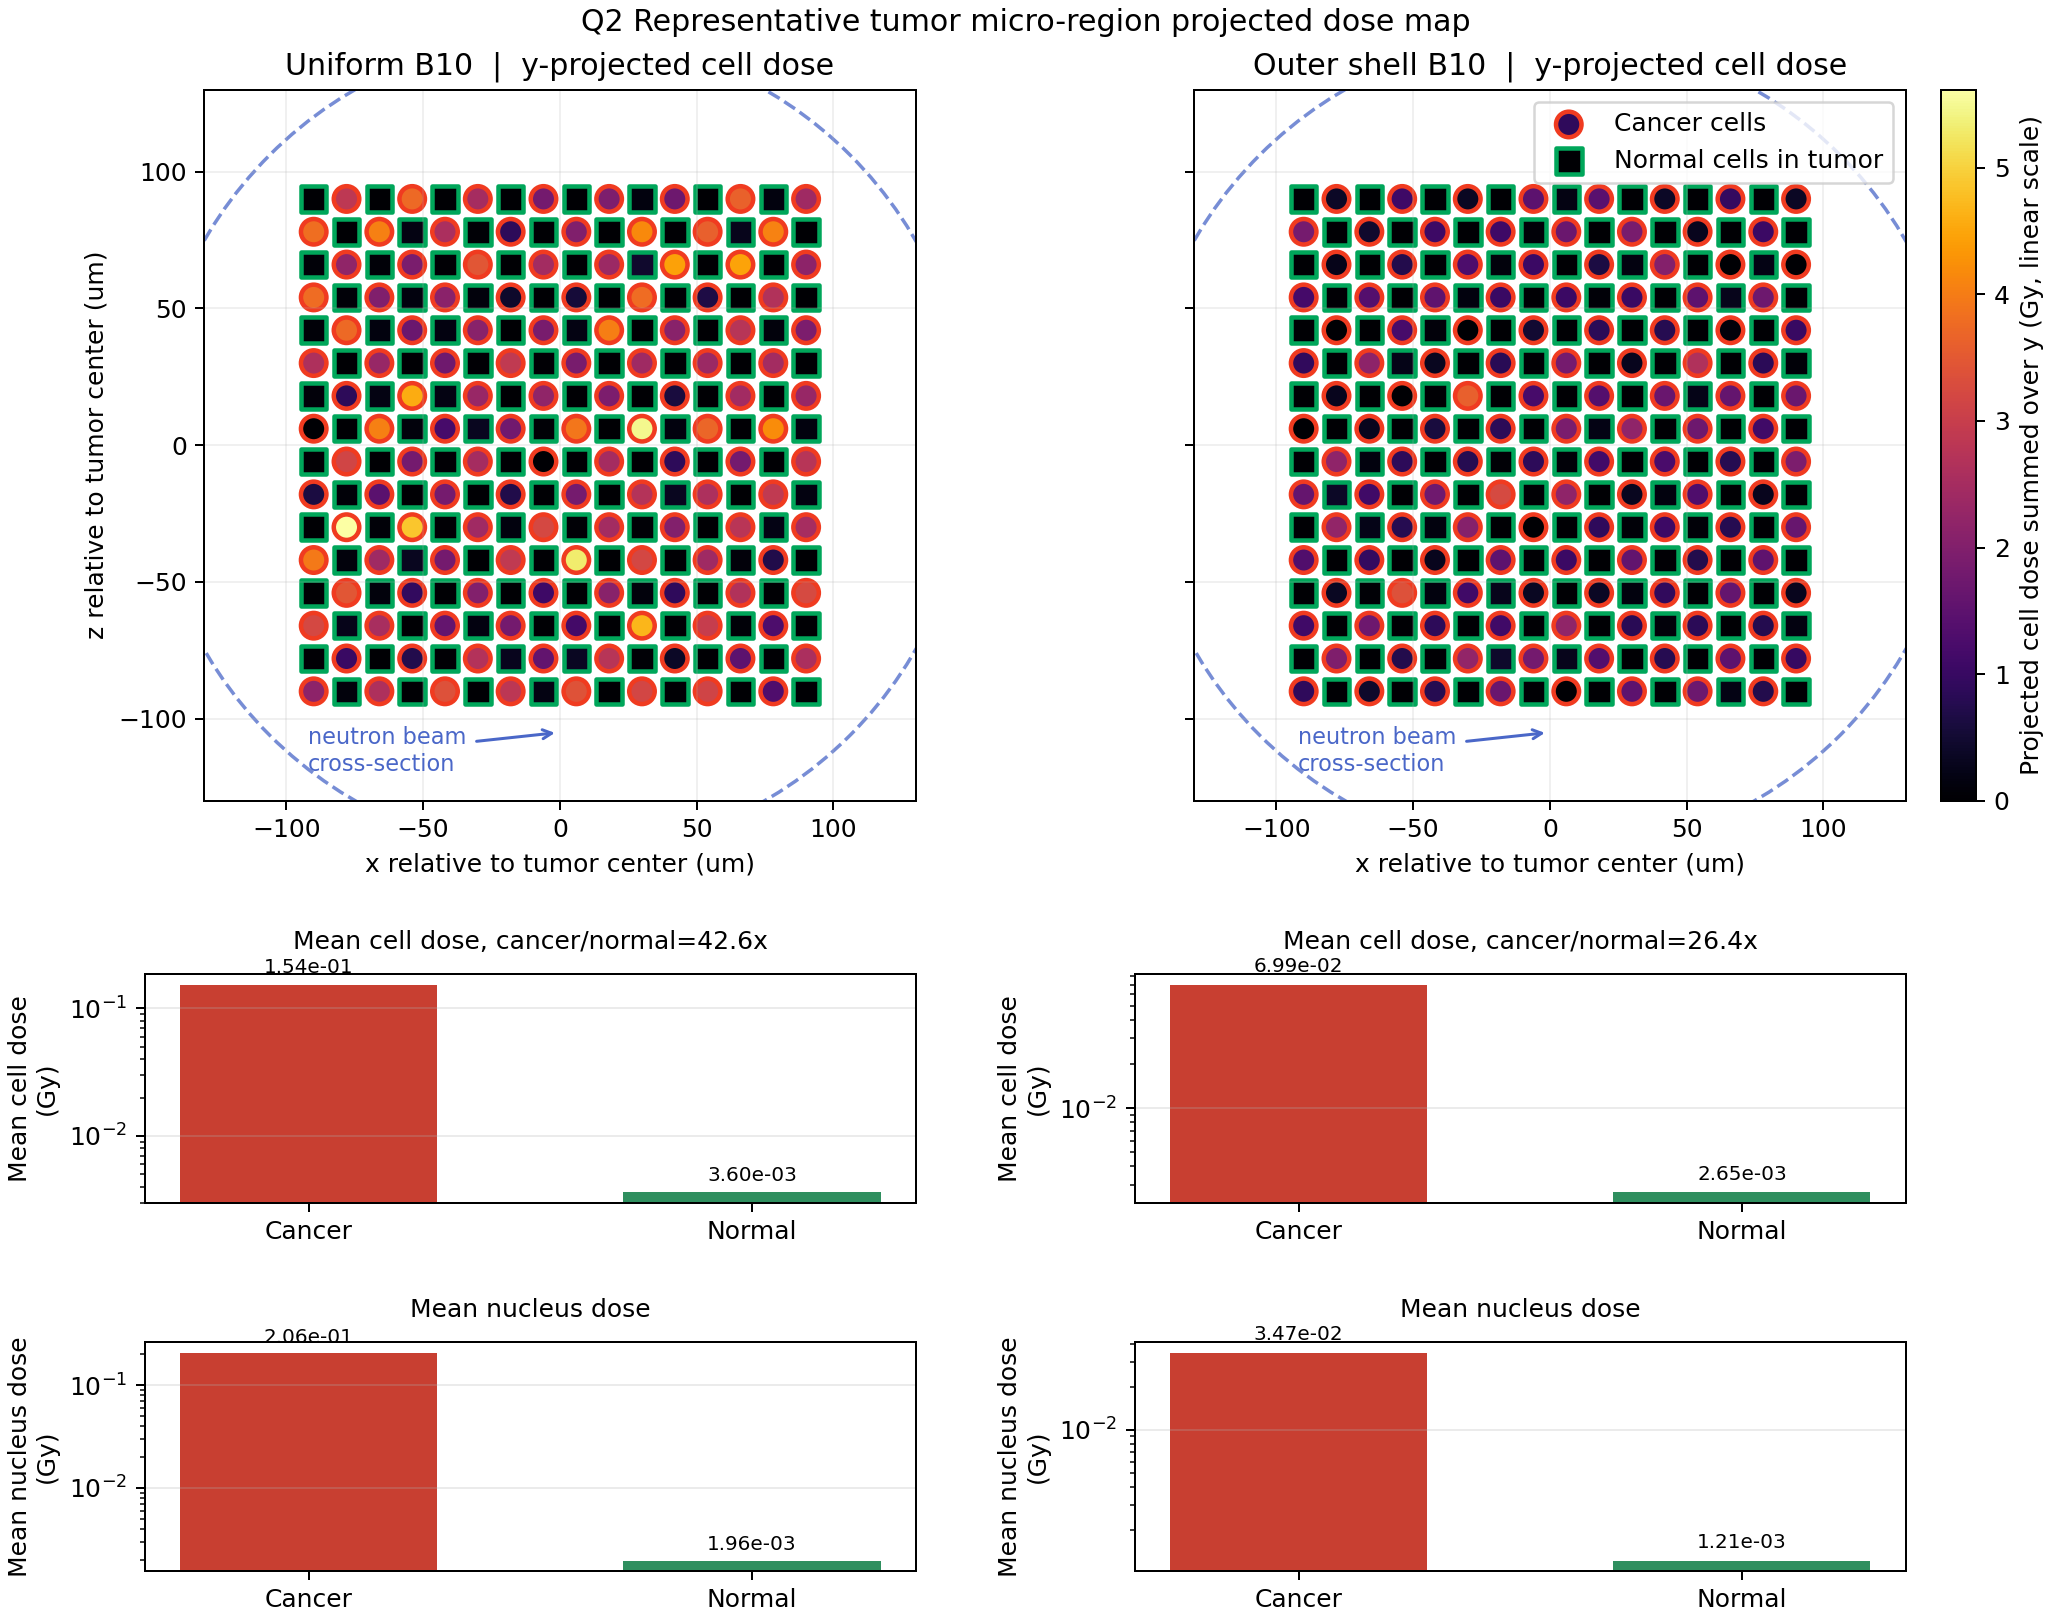
\includegraphics[width=0.9\textwidth]{Q2_micro_dose_map_uniform_vs_shell.png}
    \caption{Q2 uniform 与 shell 模式下的微区 y 投影剂量热图}
    \label{fig:q2-micro-dose}
\end{figure}

热力图中可以看到，剂量热点主要出现在含有 $^{10}\mathrm{B}$ 的肿瘤细胞柱附近，而不含硼的对照细胞区域仍有少量背景沉积。这说明当前模型中的剂量差异并不是由细胞空间位置造成的，而主要来自肿瘤细胞中额外引入的 $^{10}\mathrm{B}$。在 20 万个入射粒子下，均匀分布模式和外壳分布模式记录到的 $\alpha + ^{7}\mathrm{Li}$ 二次粒子产额分别为 1495 和 829。

具体结果如表\ref{tab:q2-fixed-dose}所示。

\begin{table}[H]
    \centering
    \caption{固定浓度下 uniform 与 shell 模式剂量比较}
    \label{tab:q2-fixed-dose}
    \small
    \begin{tabular}{lcccc}
        \toprule
        模式 & 肿瘤整细胞剂量 & 正常整细胞剂量 & 肿瘤核剂量 & 正常核剂量 \\
        \midrule
        uniform & $1.54\times 10^{-1}\,\mathrm{Gy}$ & $3.60\times 10^{-3}\,\mathrm{Gy}$ & $2.06\times 10^{-1}\,\mathrm{Gy}$ & $1.96\times 10^{-3}\,\mathrm{Gy}$ \\
        shell & $6.99\times 10^{-2}\,\mathrm{Gy}$ & $2.65\times 10^{-3}\,\mathrm{Gy}$ & $3.47\times 10^{-2}\,\mathrm{Gy}$ & $1.21\times 10^{-3}\,\mathrm{Gy}$ \\
        \bottomrule
    \end{tabular}
\end{table}

表\ref{tab:q2-fixed-dose}进一步给出了这种差异的定量表现。uniform 模式下，肿瘤整细胞剂量和肿瘤核剂量都高于 shell 模式，其中核剂量差异更明显。这与两种含硼方式的几何位置有关：uniform 模式中 $^{10}\mathrm{B}$ 分布在整个细胞体积内，短射程产物更容易在细胞核附近产生或进入核区域；shell 模式中 $^{10}\mathrm{B}$ 位于外侧壳层，产物更多沉积于壳层或细胞质附近，进入细胞核的概率相应降低。

\subsection{\texorpdfstring{$^{10}\mathrm{B}$}{10B} 浓度扫描}

固定浓度比较只能说明某一个参数点下 uniform 与 shell 的差别。为了进一步判断含硼量本身如何影响二次粒子产额、细胞核剂量和局域化比例，接下来保持中子能量不变，只扫描 $^{10}\mathrm{B}$ 浓度。每点使用 200000 个入射粒子：

\begin{center}
    \verb|1000, 3000, 10000, 30000, 100000, 300000, 500000 ppm|
\end{center}

定义剂量局域化指标：

\begin{equation}
    S_{\mathrm{cell}} =
    \frac{D_{\mathrm{tumor,cell}}}{D_{\mathrm{tumor,cell}} + D_{\mathrm{normal,cell}}},
\end{equation}

\begin{equation}
    S_{\mathrm{nucleus}} =
    \frac{D_{\mathrm{tumor,nucleus}}}{D_{\mathrm{tumor,nucleus}} + D_{\mathrm{normal,nucleus}}}.
\end{equation}

$S$ 越接近 1，剂量越集中于含 $^{10}\mathrm{B}$ 细胞。

图\ref{fig:q2-b10-scan}展示浓度扫描的四个子图：剂量局域化比例、累计细胞核剂量、$\alpha$+$^{7}\mathrm{Li}$ 产额、肿瘤核剂量与整细胞剂量之比。

\begin{figure}[H]
    \centering
    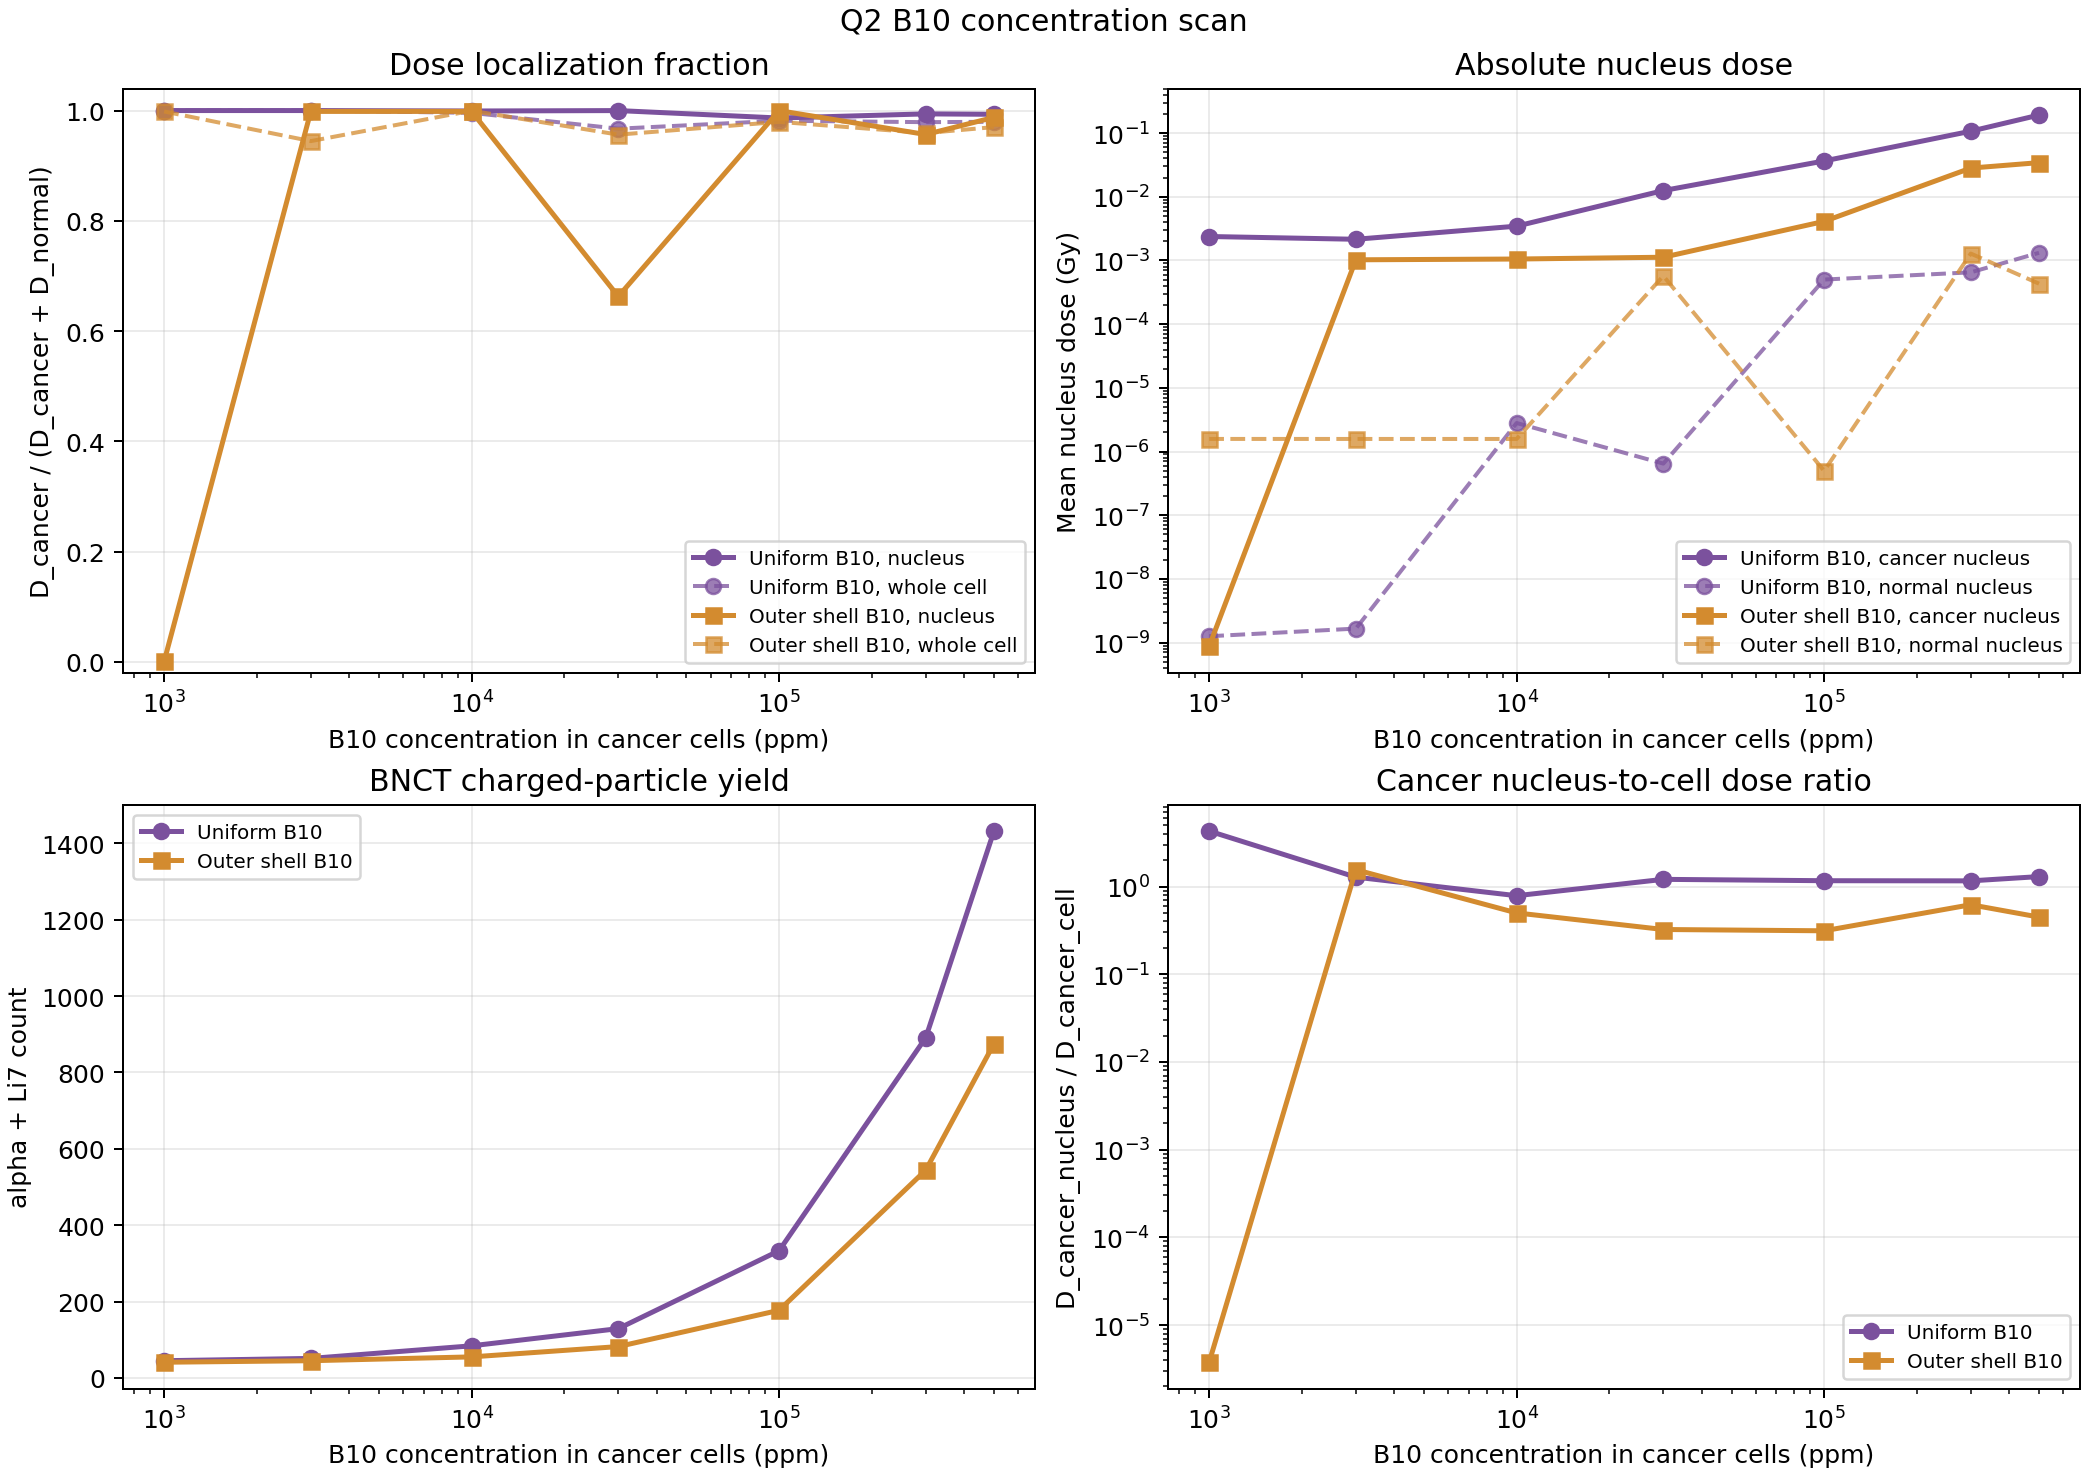
\includegraphics[width=0.92\textwidth]{Q2_b10_concentration_scan.png}
    \caption{Q2 $^{10}\mathrm{B}$ 浓度扫描}
    \label{fig:q2-b10-scan}
\end{figure}

浓度扫描中，$\alpha$+$^{7}\mathrm{Li}$ 产额随 $^{10}\mathrm{B}$ 浓度升高而增加：uniform 模式由 45 增至 1432，shell 模式由 41 增至 875。这一趋势说明，在固定中子场下，含硼量直接影响俘获反应相关的二次粒子产额，也会进一步影响含硼肿瘤细胞获得的剂量。

同时，uniform 模式的肿瘤核剂量总体高于 shell，这与固定浓度比较中的观察一致。低浓度区的局域化比例存在一定波动，主要是因为二次粒子产额较少，少数沉积事件会对平均剂量和比例指标产生较大影响。因此，这部分结果更适合用来观察浓度升高带来的整体趋势，而不适合仅凭某一个低浓度点判断最优分布。

\subsection{中子注量扫描}

浓度扫描改变的是靶细胞中可发生俘获反应的 $^{10}\mathrm{B}$ 数量。为了把这个因素和照射强度区分开，本节反过来固定 $^{10}\mathrm{B}$ 浓度为 \verb|500000 ppm|，只改变入射中子数：

\begin{center}
    \verb|2000, 5000, 10000, 20000, 50000, 100000, 200000|
\end{center}

在束斑面积和单粒子设置不变时，模拟的粒子总数与相对中子注量成正比，可直接作为中子注量的线性指标。图\ref{fig:q2-fluence-scan}展示累计剂量和二次粒子产额随注量的变化趋势。

\begin{figure}[H]
    \centering
    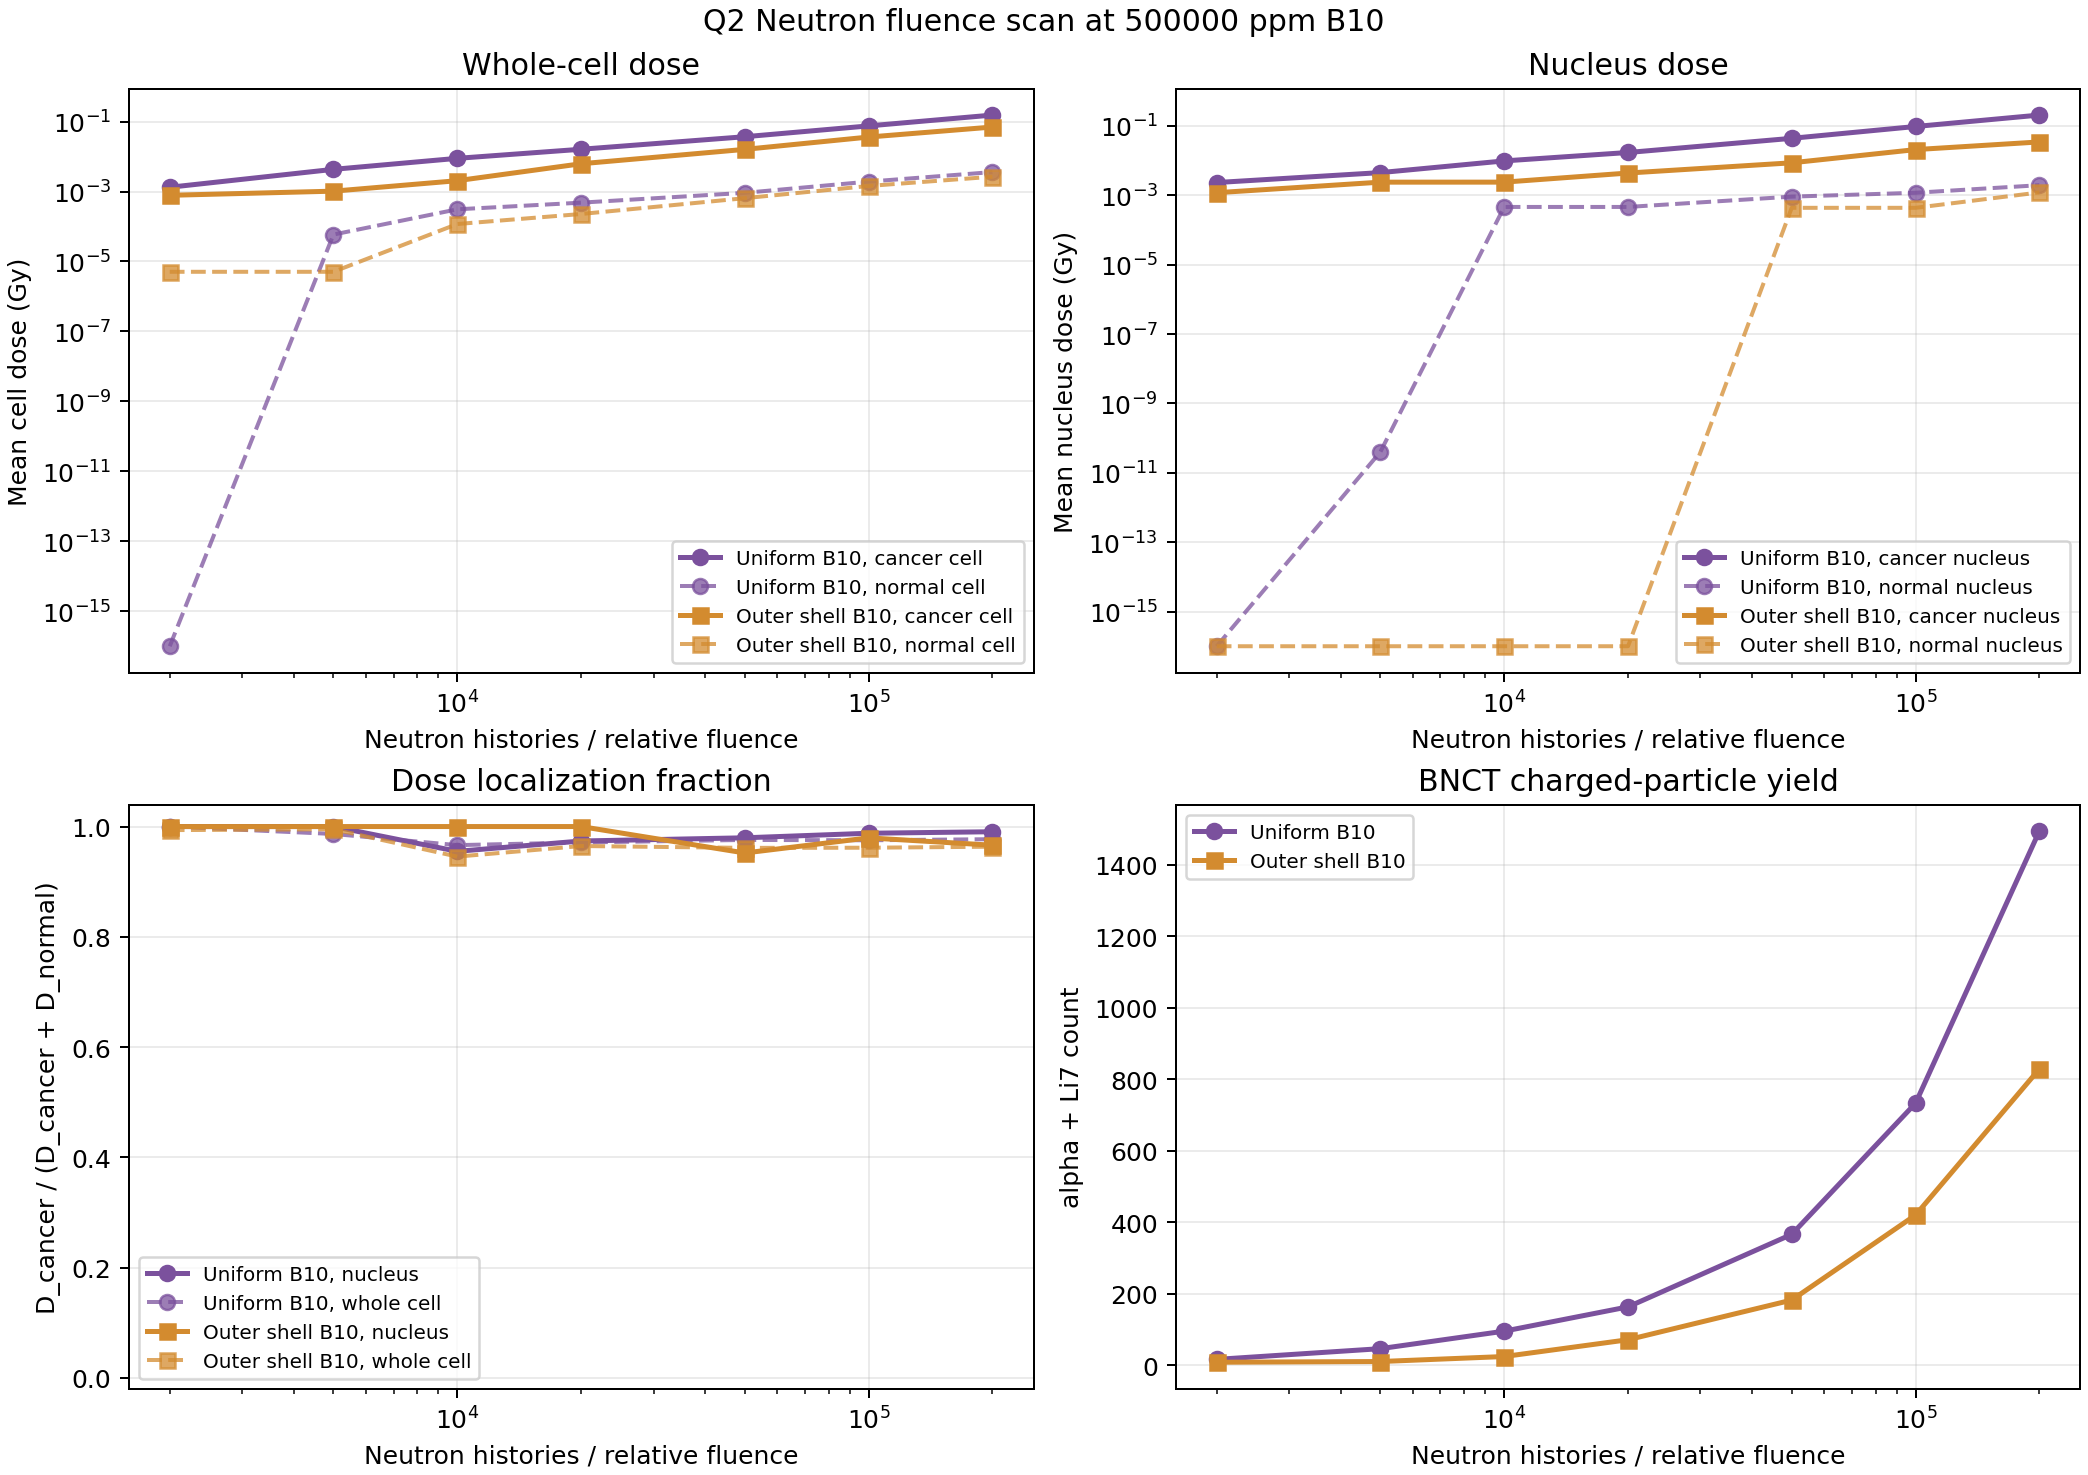
\includegraphics[width=0.92\textwidth]{Q2_neutron_fluence_scan.png}
    \caption{Q2 相对中子注量扫描}
    \label{fig:q2-fluence-scan}
\end{figure}

扫描结果中可以看到，随着粒子总数的增加，肿瘤细胞整体剂量、肿瘤细胞核剂量以及 $\alpha + ^{7}\mathrm{Li}$ 的产额均呈近似线性单调递增趋势。这说明在束斑面积、粒子能量和含硼浓度固定时，增加 histories 数主要是在增加反应机会和累计沉积能量。这一趋势与反应发生概率随入射中子注量增加的预期一致：

\begin{equation}
    R_{\mathrm{BNCT}} \approx N_{^{10}\mathrm{B}}\cdot \phi_n \cdot \sigma.
\end{equation}

但 \verb|S_cell| 与 \verb|S_nucleus| 基本维持在较高平台区域，不随入射粒子数单调变化。这一点与浓度扫描形成对比：提高中子注量会放大绝对剂量和二次粒子计数，但不会像改变 $^{10}\mathrm{B}$ 分布那样改变 tumor/normal 之间的相对选择性。

图\ref{fig:q2-fluence-maps}为不同入射粒子数下沿 $y$ 方向投影得到的热图。随注量增加，热点数量和亮度明显增加，说明更多横向位置获得了可见沉积；与此同时，对照细胞的背景剂量也会随 histories 数增加而积累。因此，在该模型中，提高中子注量更接近于增强照射强度，而不是改善含硼细胞与无硼细胞之间的剂量分离。

\begin{figure}[H]
    \centering
    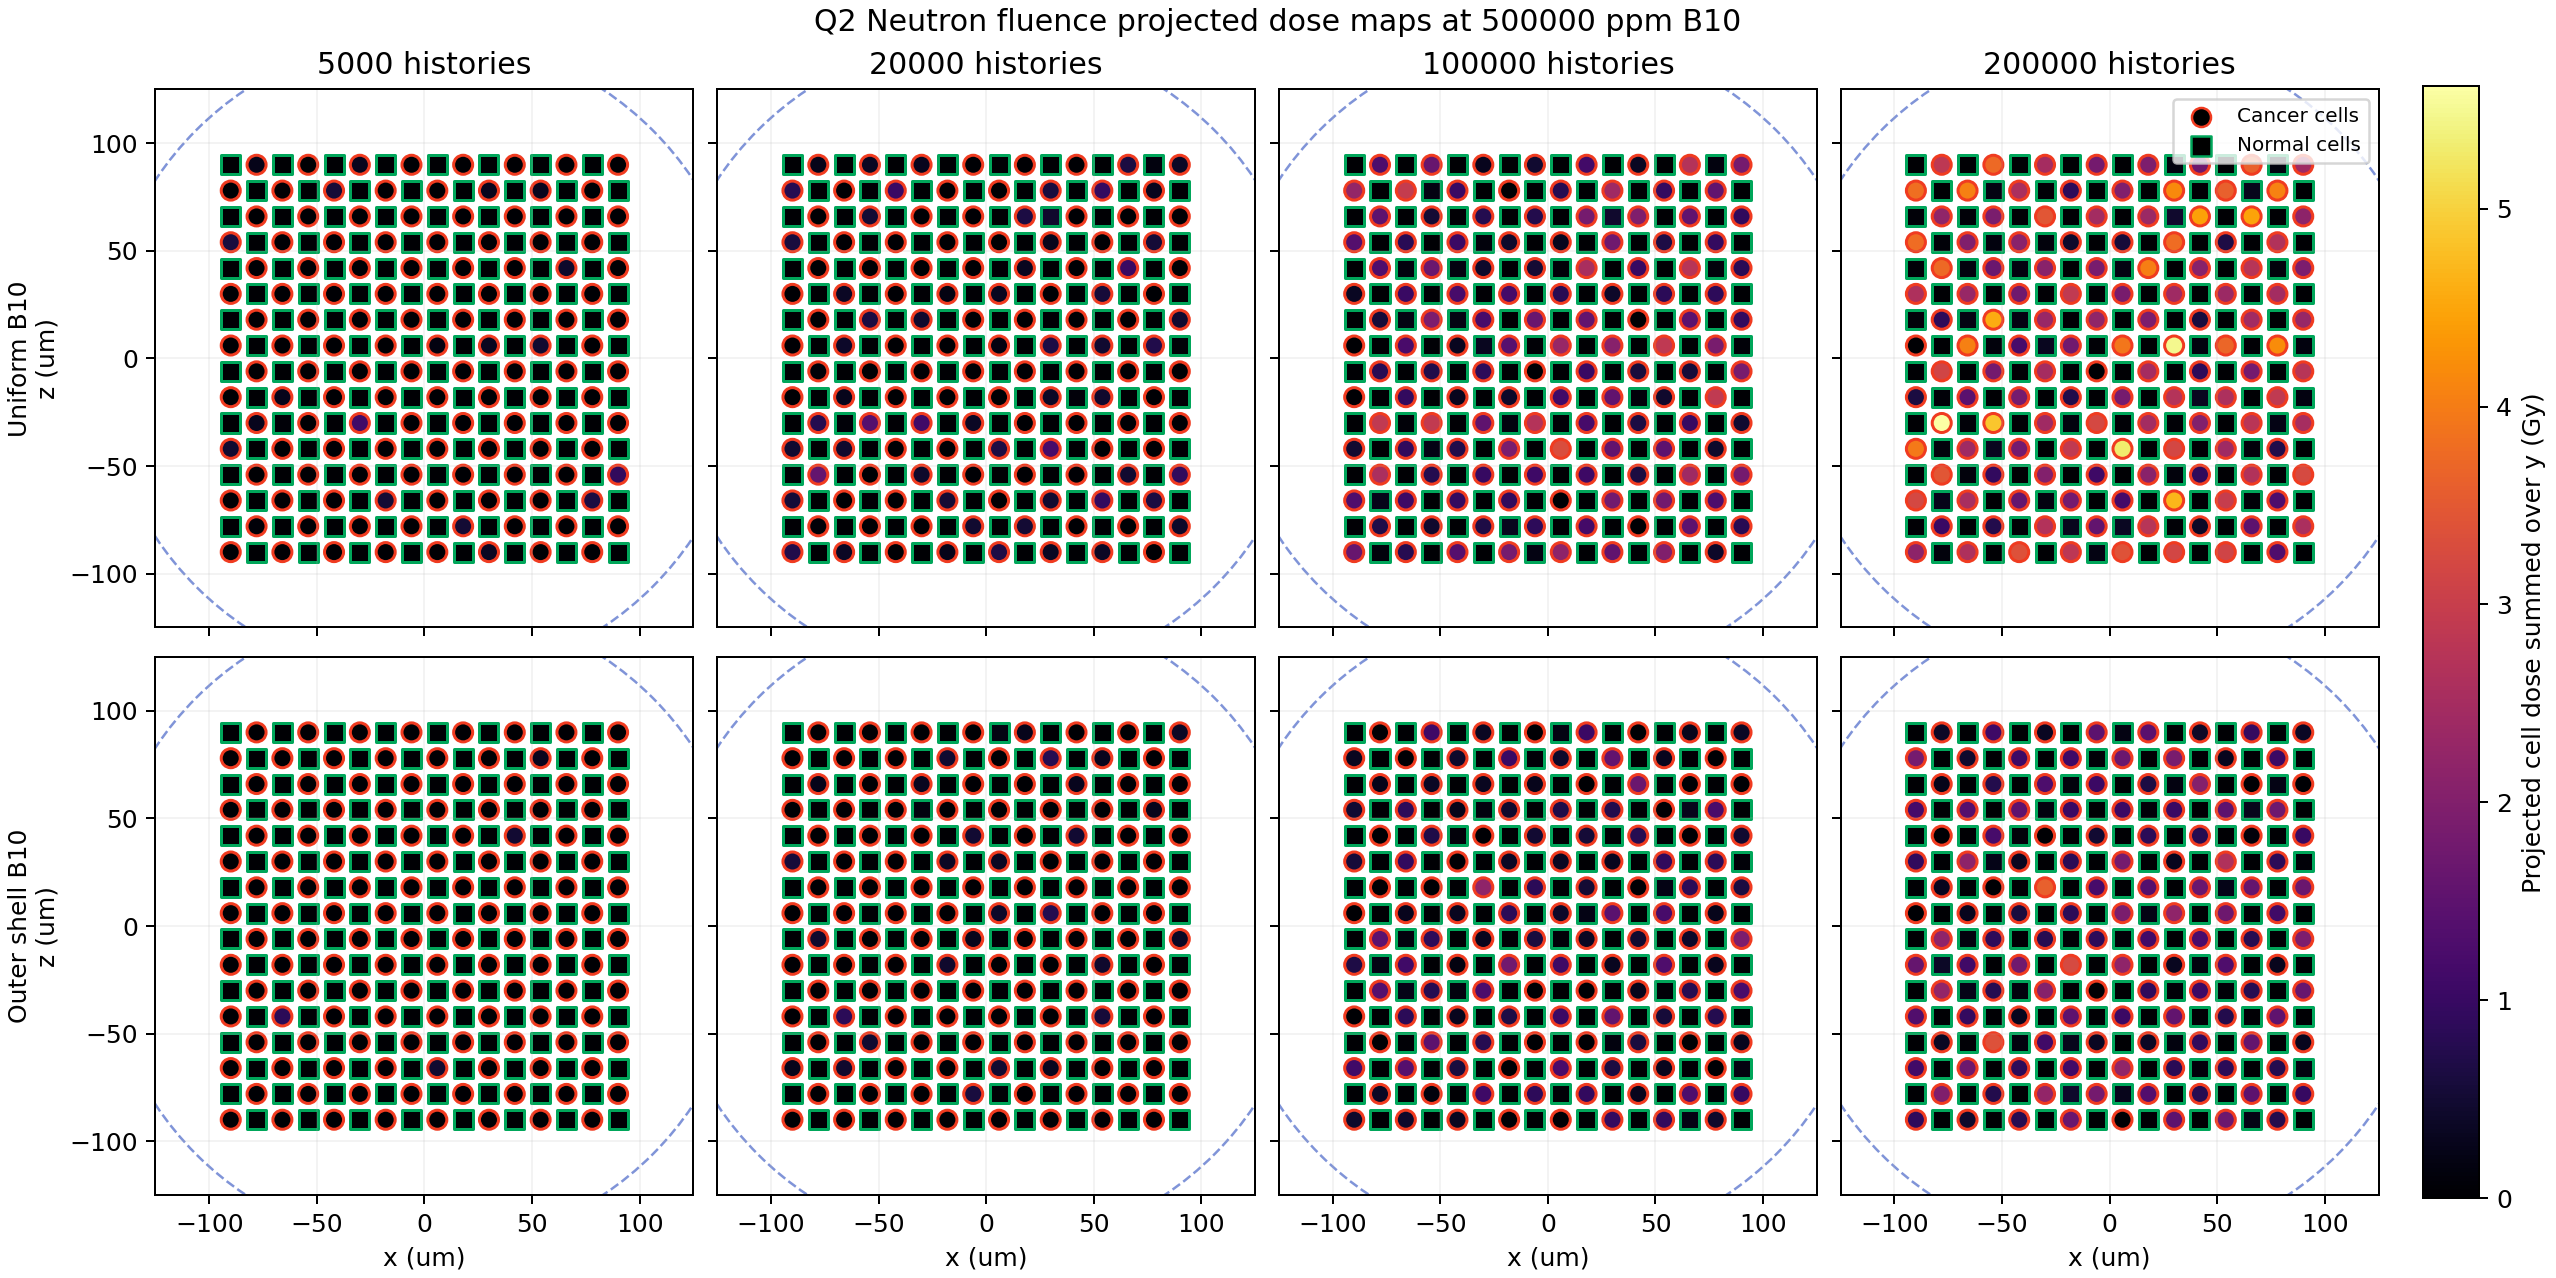
\includegraphics[width=0.92\textwidth]{Q2_neutron_fluence_projected_maps.png}
    \caption{Q2 相对中子注量扫描的投影热图}
    \label{fig:q2-fluence-maps}
\end{figure}

\subsection{BNCT 方法与 Proton/Gamma 射线对比}

前面的 Q2 分析都在 BNCT 内部比较硼分布、硼浓度和中子注量。为了把这种细胞选择性与不含硼选择性的 gamma/proton 照射放在同一微区中观察，最后补充 Q2 内部对照实验：保持同一混合细胞采样、束流位置、150 $\mu$m 束斑半径和入射数，将中子 BNCT 与 1 MeV gamma、45 MeV proton 并行比较。

\begin{table}[H]
    \centering
    \caption{Q2 不同治疗机制对照设置}
    \label{tab:q2-therapy-comparison}
    \small
    \begin{tabularx}{\textwidth}{>{\raggedright\arraybackslash}p{2.6cm}>{\raggedright\arraybackslash}X>{\raggedright\arraybackslash}p{3.2cm}>{\raggedleft\arraybackslash}p{2.0cm}}
        \toprule
        方法 & $^{10}\mathrm{B}$ 模式 & 粒子与能量 & 事件数 \\
        \midrule
        gamma & 无 & \verb|gamma 1 MeV| & \verb|20000| \\
        proton & 无 & \verb|proton 45 MeV| & \verb|20000| \\
        BNCT uniform & uniform，\verb|500000 ppm| & \verb|neutron 0.5 eV| & \verb|20000| \\
        BNCT shell & shell，\verb|500000 ppm| & \verb|neutron 0.5 eV| & \verb|20000| \\
        \bottomrule
    \end{tabularx}
\end{table}

该对照统一了几何和入射粒子数，但未统一入射总能量、处方剂量或反应类型，因此结论只限于当前设置下不同机制的物理剂量局域化趋势比较，不能作为临床治疗优劣判断。

图\ref{fig:q2-therapy-comparison}按列展示四种方法沿 $y$ 方向投影得到的热图（各自归一化色标）、分组柱状剂量比较（共享坐标轴）及整细胞局域化指标 \verb|S_cell|。

\begin{figure}[H]
    \centering
    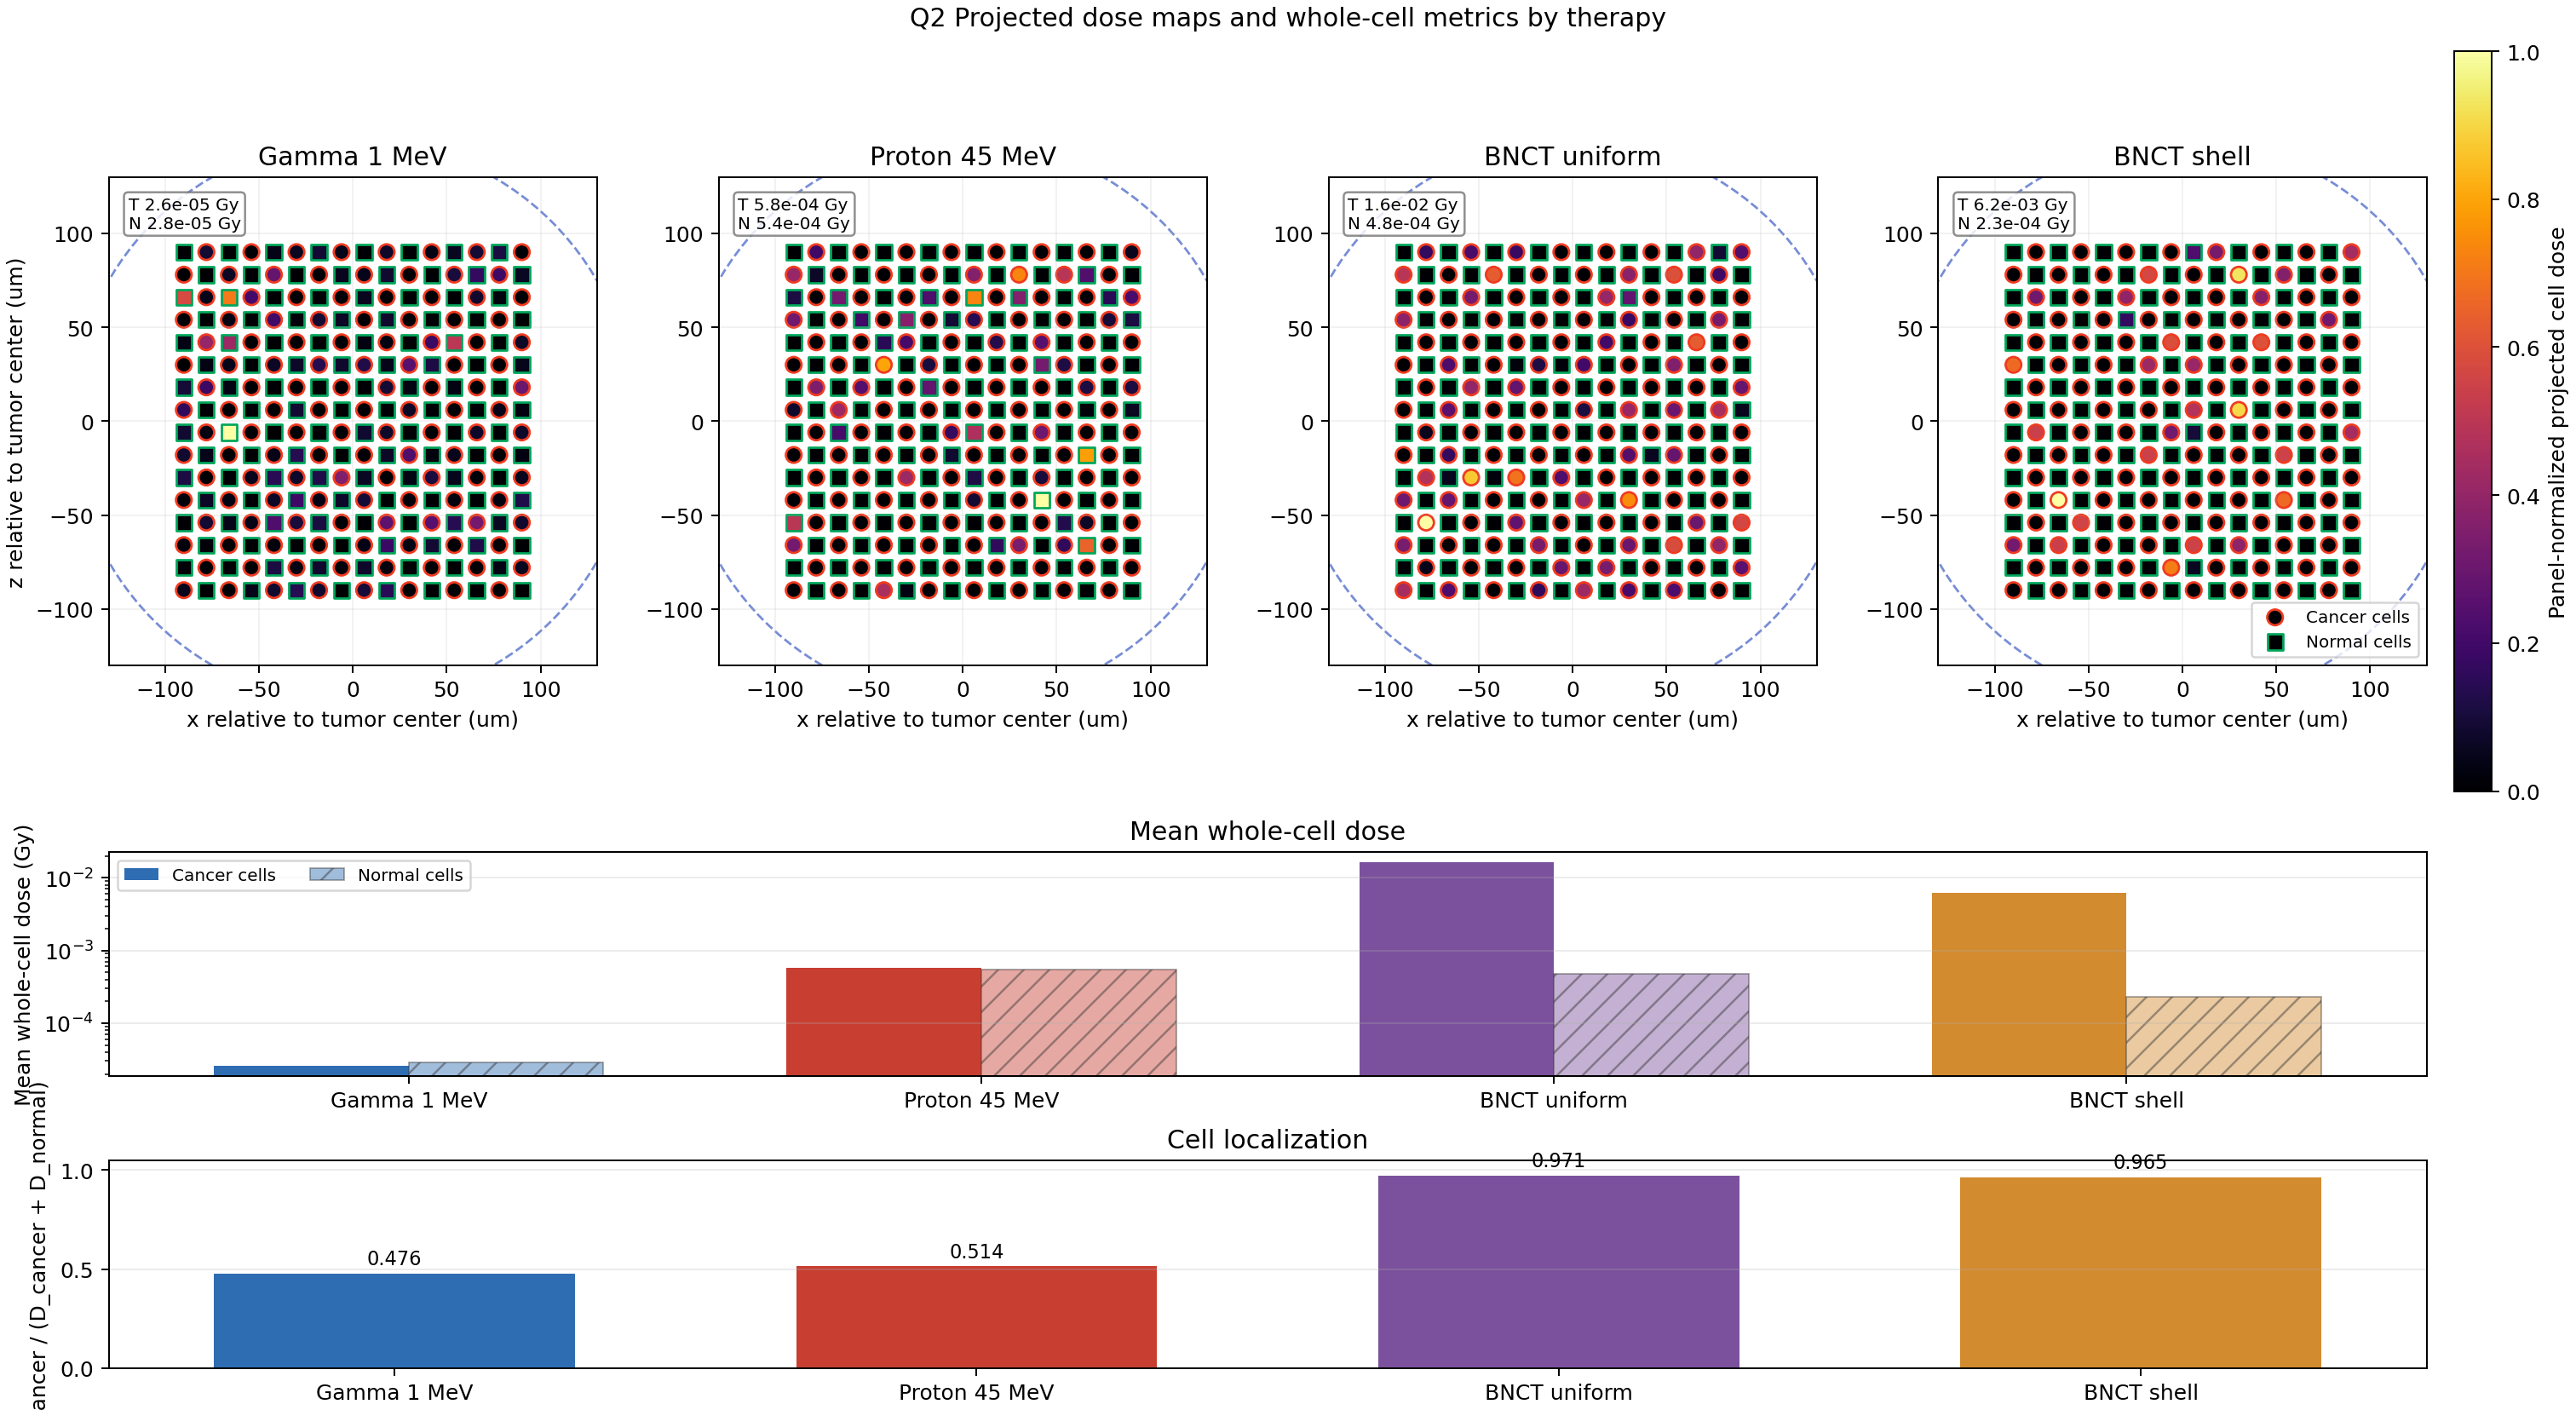
\includegraphics[width=0.95\textwidth]{Q2_therapy_comparison_projected_maps.png}
    \caption{Q2 BNCT 与 gamma/proton 的投影热图及整细胞指标对比}
    \label{fig:q2-therapy-comparison}
\end{figure}

从图中可以看到，gamma 和 proton 对两类细胞无材料选择性，肿瘤细胞与对照细胞平均剂量接近；BNCT 两组因 $^{10}\mathrm{B}$ 仅加载于肿瘤细胞，在该归一化设置下整细胞剂量局域化指标 \verb|S_cell| 更高。这里的差异主要来自模型设定中的硼富集，而不是说明 BNCT 在任意临床条件下都具有同样幅度的剂量优势。

\subsection{Q2 小结}

在本次混合细胞模型中，BNCT 的细胞选择性主要来自 $^{10}\mathrm{B}$ 只加载在肿瘤细胞这一设定。硼元素在细胞内均匀分布（uniform）时，短射程二次粒子更容易在细胞核附近沉积能量，因此肿瘤细胞核剂量高于外壳分布（shell）。中子注量主要改变累计剂量大小，而细胞选择性的变化更多由 $^{10}\mathrm{B}$ 的富集和分布方式决定。

\section{结论}

本项目完成了从简化人体 Gamma/Proton 照射到微观细胞 BNCT 计分的 Geant4 模拟。

Q1：在本模型中，gamma 能量沉积较为弥散，未出现明显峰值；proton 可通过能量调节改变 Bragg peak 位置，45 MeV 在当前几何和扫描点中与肿瘤深度匹配较好。

Q2：在 $^{10}\mathrm{B}$ 仅富集于肿瘤细胞的理想模型中，$\alpha$/$^{7}\mathrm{Li}$ 短射程产物使剂量更多集中在含硼细胞附近；$^{10}\mathrm{B}$ 浓度影响反应活性与靶细胞剂量，uniform 分布在当前参数下更有利于提高肿瘤核剂量；相对中子注量主要控制累计剂量和二次粒子产额，对由 $^{10}\mathrm{B}$ 分布决定的细胞选择性改变较小。

因此，本报告中的结果更适合作为 Geant4 建模和计分流程的展示，而不是临床剂量结论。若继续推进，需要进一步引入真实组织材料、实际硼药物摄取分布、重复统计、RBE 修正和细胞生存模型。

\section{局限性}

虽然模型能够反映一些预期中的物理趋势，但结果不能直接等同于临床真实情况。首先，整个三维人体模型全部用纯水代替，忽视了骨骼、肺部和脂肪等真实组织对粒子输运、散射与衰减的影响。同时，Q1 宏观剂量的事件数有限，Bragg 峰附近的曲线形状仍然比较粗糙。

其次，Q2 的材料与浓度设定偏离临床。为了在微观模拟中获得可见的增强信号，本报告采用了极高的硼浓度（500000 ppm），并假设正常对照细胞完全不吸附硼，因此会高估细胞选择性。不同粒子对照时也未统一入射总能量或处方剂量，当前结果只适合定性比较物理剂量局域化趋势。模型中还没有引入 RBE（相对生物效应）修正、DNA 损伤模型或细胞存活曲线；对于 proton，也未考虑真实治疗计划中的射程不确定性、展宽 Bragg peak 和组织不均匀性。因此，本报告不能直接外推为实际细胞杀伤率或临床治疗优劣。

\begin{thebibliography}{9}

\bibitem{desai2020gamma}
Desai R, Rich KM.
Therapeutic Role of Gamma Knife Stereotactic Radiosurgery in Neuro-Oncology.
\textit{Missouri Medicine}. 2020;117(1):33--38.

\bibitem{mohan2022proton}
Mohan R.
A Review of Proton Therapy -- Current Status and Future Directions.
\textit{Precision Radiation Oncology}. 2022;6(2):164--176.
doi:10.1002/pro6.1149.

\bibitem{nedunchezhian2016bnct}
Nedunchezhian K, Aswath N, Thiruppathy M, Thirugnanamurthy S.
Boron Neutron Capture Therapy -- A Literature Review.
\textit{Journal of Clinical and Diagnostic Research}. 2016;10(12):ZE01--ZE04.
doi:10.7860/JCDR/2016/19890.9024.

\end{thebibliography}

\end{document}
